This appendix provides more related work, supplementary discussions, proofs, and experiments to support the main text. We organize the appendix as follows:
\begin{itemize}
    \item \textbf{Section~\ref{app:additional related work}}: Summarizes additional related work.  

    \item \textbf{Section~\ref{app:proof of prop1}}: Provides the proof of Proposition~\ref{prop: prob_guaranee_for_part_1_1} (probabilistic guarantee for part 1).

    \item \textbf{Section~\ref{mgm}}: Explains the role of sample size in Part 1 Step 1 and its effect on $\boldsymbol{v}_{\max}$.  

    \item \textbf{Section~\ref{app:proof of prop2}}: Gives the proof of Proposition~\ref{prop: sound_verification_2} (NMS Soundness Verification).

    \item \textbf{Section~\ref{app:ll1}}: Proves Lemma~\ref{lemma: threshold_prop_1} (threshold properties).

    \item \textbf{Section~\ref{app:ll2}}: Proves Lemma~\ref{lemma: threshold_computaion_2} (explicit threshold computation formulas).

    \item \textbf{Section~\ref{app:verification bound}}: Defines and estimates the verification bound for object detection and provides proofs for Lemmas~\ref{ll3} and \ref{ll4}.


    \item \textbf{Section~\ref{app:nms}}: Details the verification procedure for Non-Maximum Suppression, including abstract box construction and IoU bound computation.  
    

    \item \textbf{Section~\ref{app:th1}}: Proves Theorem~\ref{theorem: part_3_guarantee_1} (probabilistic guarantee for Part 3).  


    \item \textbf{Section~\ref{app:part3}}: We propose a strict sound gradient-based refinement algorithm to implement Part Three on small-scale networks(Theorem~\ref{ths}).
    % Discusses the application of Part Three on small-scale networks and provides the corresponding gradient-based refinement algorithm.

    \item \textbf{Section~\ref{app:th3}}: Provides the proof of Theorem~\ref{ths} based on dual formulations.  


    \item \textbf{Section~\ref{app:theorem2}}: Gives the proof of Theorem~\ref{theorem:  full_guarateen_2}, combining probabilistic guarantees across all parts.  

    \item \textbf{Section~\ref{app:exp details}}: Reports detailed experimental settings, sample number calculations, and server configuration.  

    \item \textbf{Section~\ref{app:efficiency of nms}}: Discuss the efficiency of the NMS verification process.

    \item \textbf{Section~\ref{app:part3 effect}}: Shows the effectiveness of Part 3 refinement for YOLO and CNNs.  

    \item \textbf{Section~\ref{app:time comparison}}: Shows time-verified box comparison between our method and $\mathrm{RCP}_N$.

    \item \textbf{Section~\ref{app:real world}}: Demonstrates our method's effectiveness on real-world images. 

    \item \textbf{Section~\ref{app:median}}: Compares our method against median smoothing under Gaussian noise.  

    \item \textbf{Section~\ref{app:ablation}}: Presents an ablation study on parameters $\eta$ and $\iota$.  

    \item \textbf{Section~\ref{app:border}}: Discusses the broader impact of our verification method.  

    \item \textbf{Section~\ref{app:llm}} : LLM Usage Statement.
    
    \item \textbf{Section~\ref{app:hyperprameters}}: Lists and explains all hyperparameters used in our algorithms.

    \item \textbf{Section~\ref{app: other_attack}}: Provides details on how to adapt our method to other attacks beyond OD attacks.
\end{itemize}

\section{Additional Related Work}
\label{app:additional related work}
\paragraph{Adversarial attacks.}
Adversarial methods induce misclassification through imperceptible perturbations. White-box attacks exploit gradient information~\citep{goodfellow2015explaining,madry2018towards,carlini2017towards} and can be adapted to OD attacks~\citep{choi2022adversarial,li2020qeba}. Black-box attacks use transferability~\citep{chen2024theory} or query-based optimization~\citep{li2020qeba}; these are more practical but may be computationally costly. 
Using adversarial attacks in isolation only demonstrates non-robustness if the attack is successful, whereas our method provides a rigorous probabilistic certificate of robustness. A network that is robust with high probability under common perturbations(e.g. sensor noise) is acceptable for practical deployment, whereas the strict requirement of complete robustness in a neighborhood often leads to a significant drop in network performance. Thus focus is on providing probabilistic robustness under realistic perturbations such as sensor noise rather than adversarial attacks (which often represent worst-case scenarios).
\paragraph{Bound Estimate Methods.} 
There are several classical methods for estimating probabilistic output bounds of neural networks, including DKW-based confidence regions~\citep{massart1990tight,naaman2021tight}, ERM-based hyper-rectangles, and $\epsilon$-nets~\citep{haussler1987netsAS, blohm2025probably}. While these methods are theoretically robust, their sample complexity typically scales with the output dimension $d_L$ (e.g., $\tilde{O}(d_L/\epsilon)$ for $\epsilon$-nets). Given the extremely high-dimensional output space of YOLO networks, dimension-dependent bounds like those from $\epsilon$-nets or DKW would be computationally infeasible. We chose this trade-off—sacrificing some transparency in the shape of the confidence region—to ensure scalability.
\paragraph{PAC with Attack.} There are several PAC verification methods that incorporate adversarial attacks to refine the estimated output bounds~\citep{blohm2025probably,li2022towards,baluta2021scalable}. For example, \cite{blohm2025probably} evaluates the robustness of individual points via a local robustness oracle (such as PGD or LiRPA) and leverages $\epsilon$-net sampling methods to provide high-probability statistical guarantees for global robustness. Combining attacks with PAC verification is an interesting direction, we will explore this in future work.

\section{The proof of Proposition~\ref{prop: prob_guaranee_for_part_1_1}}
\label{app:proof of prop1}
\begin{boxedenv}[]
\begin{prop*}[probabilistic guarantee for part 1]
For any $N_1>1$, let $\boldsymbol{v}_{\max}$ be a vector with positive components (e.g., as estimated from $N_1$ samples in Algorithm~\ref{algforp1}). If $c_1$ is computed based on this $\boldsymbol{v}_{\max}$ using $N_2\ge [\frac{2\ln 1/\beta}{\alpha}+2+\frac{2\ln2/\alpha}{\alpha}]$ samples as described in Algorithm~\ref{algforp1},
then with probability $1-\beta$, we have: $\mathrm{P}_{\boldsymbol{x}\sim \mathcal{C}}\left(|\F(\boldsymbol{x})-\F(\boldsymbol{x}^{(0)})|\le c_1 \cdot \boldsymbol{v}_{\max} \right)\ge 1-\alpha$, which implies $\mathrm{P}_{\boldsymbol{x}\sim \mathcal{C}}\left(\F(\boldsymbol{x})\in \mathcal{Z} \right)\ge 1-\alpha$.
\end{prop*}
\end{boxedenv}




This proposition can be directly obtained by classic method $\mathrm{RCP}_N$, which is introduced below.
\subsection{Classic method for probability sampling.}
\label{app:rcp}
We begin by introducing a well-known result from the $\mathrm{RCP}_N$ method~\citep{campi2009scenario}, which forms the basis of our approach in this section.
Consider the following optimization problem with an infinite number of constraints:
\begin{equation}
\label{eq:RCP_N origin}
\min_{\boldsymbol{x}\in \R^d} \boldsymbol{a}^{\top}\boldsymbol{x}+{b}\quad \mathrm{s.t.} \quad \boldsymbol{x}\in \cap_{\delta\in\Delta}\mathcal{X}_{\delta},
\end{equation}
where $\Delta$ is an index set, and $\mathcal{X}_{\delta}\subseteq\R^d$ denotes the constraint set corresponding to the index $\delta$.

Since the constraints are infinite, we can not solve the problem directly. Thus we consider sample the constraints $\{\delta_i\}_{i=1}^N$ from $\Delta$, and estimate the possibility that the optimal value of the optimization problem \eqref{eq:RCP_N sample} with the constraints $\{\mathcal{X}_{\delta_i}\}_{i=1}^N$ is the optimal value of the problem \eqref{eq:RCP_N origin} with the constraints $\{\mathcal{X}_{\delta}\}_{\delta\in\Delta}$. 

\begin{equation}
\label{eq:RCP_N sample}
\min_{\boldsymbol{x}\in \R^d} \boldsymbol{a}^{\top} \boldsymbol{x}+b \ \
\mathrm{s.t.} \ \ \boldsymbol{x}\in\cap_{\delta_i,i\in[N]}\mathcal{X}_{\delta_i}
\end{equation}

When $X_{\delta}$ is convex for every $\delta\in\Delta$, we have that: 
If $\mathcal{Q}$ is a distribution defined on $\Delta$, and $N\ge[\frac{2\ln (1/\beta)}{\alpha}+2d+\frac{2d\ln(2/\alpha)}{\alpha}]$, then with probability $1-\beta$ of $\{\delta_i\}_{i=1}^N\sim \mathcal{Q}$, if the following optimization problem \eqref{eq:RCP_N sample} has a unique solution $\boldsymbol{x}_{\min}$, such solution $\boldsymbol{x}_{\min}$ satisfies $\mathrm{P}_{\delta\sim \Delta}(\boldsymbol{x}_{\min}\in \mathcal{X}_{\delta})\ge1-\alpha$. 

A classic application of $\mathrm{RCP}_N$ is to find the Essential Supremum of a function $f(t)$ over a domain $\Delta$. This can be formulated as an optimization problem with a decision variable $x \in \mathbb{R}$ (i.e., dimension $d=1$):
\begin{equation}
\label{eq:RCP_N originda}
\min_{x\in \R} x \quad \mathrm{s.t.} \quad x \ge f(t), \ \forall t\in\Delta.
\end{equation}
By applying the $\mathrm{RCP}_N$ result with $d=1$, we know that if we draw $N$ samples $\{t_i\}_{i=1}^N$ from $\Delta$, where
\[
N \ge \left\lceil \frac{2\ln (1/\beta)}{\alpha} + 2 + \frac{2\ln(2/\alpha)}{\alpha} \right\rceil,
\]
then with probability at least $1-\beta$, we have:
$
\mathrm{P}_{t\sim \Delta}\left(f(t)\le \max_{i=1,\dots,N}\{f(t_i)\}\right) \ge 1-\alpha.
$

\section{Analysis of the Sample Size Effect in Part 1 Step 1}
\label{mgm}

In this section, we justify the choice of $\boldsymbol{v}_{\max}$ as presented in Algorithm~\ref{algforp1}. The main objective is to ensure that the range $\mathcal{Z}$ obtained by Algorithm~\ref{algforp1} does not significantly exceed the actual range $\{\F(\boldsymbol{x})\}_{\boldsymbol{x} \in \mathcal{C}}$.

Algorithm~\ref{algforp1} guarantees this property under certain assumptions, as detailed in the following proposition.

\begin{prop}
    Let $|(\F(\boldsymbol{x}))_i-(\F(\boldsymbol{x}^{(0)}))_i|\sim N_i$ when $x\sim \mathcal{C}$, and $v_i\in\R_+$ is the minimum value such that $\mathrm{P}_{x\sim N_i}(x\le v_i)=1$. 
    
    If $\alpha^i_1\le\alpha^i_2\le1$ and $\beta_1,\beta_2$ satisfy that: $\mathrm{P}_{x\sim N_i}(x\le \alpha^i_1v_i)=\beta_1$ and $\mathrm{P}_{x\sim N_i}(x\le \alpha^i_2v_i)=\beta_2$ for any $i\in[d_L]$.

Let $z_i=(c_1\boldsymbol{v}_{\max})_i$ where $c_1$ and $\boldsymbol{v}_{\max}$ are obtained by algorithm \ref{algforp1}, then we have that: $ \frac{z_j}{v_j}\le \max_i\{\frac{\alpha^i_2}{\alpha^i_1}\}\alpha^j_2$ for any $j\in[d_L]$ with probability $1-d_L(1+\beta^{N_1}_1-\beta^{N_1}_2)-d_L(1+\beta^{N_2}_1-\beta^{N_2}_2)$.
\end{prop}

% \begin{proof}
%     Easy to see that, for any $i\in[d_L]$, for the random selected  $N_1$ points $\{x_j\}$ in $\mathcal{C}$ in algorithm \ref{algforp1}, there are $\mathrm{P}(\alpha^i_2v_i\ge \max_j (x_j)_i\ge \alpha^i_1v_i)\ge -\beta^{N_1}_1+\beta^{N_1}_2$ for any $i\in[d_L]$. So with probability $1-d_L(1+\beta^{N_1}_1-\beta^{N_1}_2)$, there are $\alpha^i_2v_i\ge \max_j (x_j)_i\ge \alpha^i_1v_i$ stand for any $i\in[d_L]$.

% Similar, for the $N_2$ points $\{x'_j\}$ random selected in the algorithm \ref{algforp1},  with probability $1-d_L(1+\beta^{N_2}_1-\beta^{N_2}_2)$, there are $\alpha^i_2v_i\ge \max_j (x'_j)_i\ge \alpha^i_1v_i$ stand for any $i\in[d_L]$.

%     Hence, based on the algorithm \ref{algforp1}, we know that $c_1\le \max_i\{\alpha_2^i/\alpha^i_1\}$ when the above results hold for any $i\in[d_L]$. Hence, there are $(c_1\boldsymbol{v}_{\max})_j\le \max_i\{\frac{\alpha^i_2}{\alpha^i_1}\}\alpha^j_2v_j$ any $j\in[d_L]$, which is what we want.    
% \end{proof}
\begin{proof}
    Observe that for any coordinate $i \in [d_L]$, given the $N_1$ randomly selected points $\{x_k\}$ from $\mathcal{C}$ in Algorithm~\ref{algforp1}, we have:
    \[
    \mathrm{P}\left(\alpha^i_2 v_i \ge \max_k (x_k)_i \ge \alpha^i_1 v_i\right) \ge \beta^{N_1}_2 - \beta^{N_1}_1.
    \]
    Applying the union bound, with probability $1 - d_L(1 - (\beta^{N_1}_2 - \beta^{N_1}_1)) = 1 - d_L(1 + \beta^{N_1}_1 - \beta^{N_1}_2)$, the condition $\alpha^i_2 v_i \ge \max_k (x_k)_i \ge \alpha^i_1 v_i$ holds for all $i \in [d_L]$.

    Similarly, for the $N_2$ points $\{x'_k\}$ randomly selected in Algorithm~\ref{algforp1}, with probability $1 - d_L(1 + \beta^{N_2}_1 - \beta^{N_2}_2)$, the condition $\alpha^i_2 v_i \ge \max_k (x'_k)_i \ge \alpha^i_1 v_i$ holds for all $i \in [d_L]$.

    Consequently, based on the construction in Algorithm~\ref{algforp1}, if the above events occur, we have $c_1 \le \max_i \{\alpha_2^i / \alpha^i_1\}$. Therefore, for any $j \in [d_L]$, implies:
    \[
    (c_1\boldsymbol{v}_{\max})_j \le \max_i \left\{\frac{\alpha^i_2}{\alpha^i_1}\right\} \alpha^j_2 v_j,
    \]
    which completes the proof.
\end{proof}

% Based on our observations of many neural network outputs, we have found that the outputs of neural networks are highly likely to be concentrated in a certain region. An  example is given in the figure \ref{fig:toefine}. Based on this, there can be $\alpha_1\approx\alpha_2$ but $1\approx\beta_2$ and $1>\beta_1$. Hence, because $\alpha_1\approx\alpha_2$, we know each dimension of $\mathcal{Z}$ will not far beyond $v_i$; because $1\approx\beta_2$ and $1>\beta_1$, we know $1-d_L(1+\beta^{N_1}_1-\beta^{N_1}_2)-d_L(1+\beta^{N_2}_1-\beta^{N_2}_2)\approx1$, which is what we want. 


% However, in reality, we cannot accurately estimate $\alpha_i$ and $\beta_i$, so the choice of $N_1$ is mainly determined by experiments. The above theorem is only used to support the accuracy of $\mathcal{Z}$ we found when $N_1$ is sufficiently large.

Based on our observations of numerous neural network outputs, we find that the output values are highly likely to be concentrated within a specific region. An example is provided in Figure~\ref{fig:toefine}. Based on this observation, it is possible that $\alpha_1 \approx \alpha_2$ while $\beta_2 \approx 1$ and $\beta_1 < 1$.
Consequently, since $\alpha_1 \approx \alpha_2$, we can infer that each dimension of $\mathcal{Z}$ will not extend significantly beyond $v_i$. Furthermore, since $\beta_2 \approx 1$ and $\beta_1 < 1$, the probability term satisfies:
\[
1 - d_L(1+\beta^{N_1}_1-\beta^{N_1}_2) - d_L(1+\beta^{N_2}_1-\beta^{N_2}_2) \approx 1.
\]

However, in practice, we cannot accurately estimate $\alpha_i$ and $\beta_i$. Therefore, the choice of $N_1$ is primarily determined empirically. The theorem above serves to theoretically justify the accuracy of the region $\mathcal{Z}$ obtained when $N_1$ is sufficiently large.

\begin{figure}[!t]
    \centering
    \includegraphics[width=0.6\textwidth]{image/_20250513202210.png}
    \caption{This is a picture about the distribution around a sample $x$. 
 When we take $\alpha_1=2.3/3.5$ and $\alpha_2=2.8/3.5$, by such figure, we have that $\beta_1\le0.99$ but $\beta_2\approx1$. Thus $(\alpha_2/\alpha_1)\alpha_2\approx 0.97$. Hence, if there are $N_1=N_2=3000$, then $1-d_L(1+\beta^{N_1}_1-\beta^{N_1}_2)-d_L(1+\beta^{N_2}_1-\beta^{N_2}_2)\ge0.99$ when $d_L\le 10^7$.}
      \label{fig:yolo_1_255_appendix}

    \label{fig:toefine}
\end{figure}



\section{The proof of Proposition~\ref{prop: sound_verification_2}}
\label{app:proof of prop2}

\begin{boxedenv}[]
\begin{prop*}[NMS Soundness Verification]
For given $\mathcal{Z}$, $\tau$, and $box_{\mathrm{gt}}$, if $Q(\mathcal{Z},\tau,box_{\mathrm{gt}}) \neq \emptyset$, then for $\forall k\in\Delta: \exists box_i\in\mathrm{N}(\boldsymbol{z}^k),$ $s.t. \mathrm{IoU}(box_i,box_{\mathrm{gt}})\ge\tau \land \mathrm{Class}(box_i)=\mathrm{Class}(box_{\mathrm{gt}})$.
\end{prop*}
\end{boxedenv}

\label{app:pp1}
We first present a lemma.
\begin{lemma}
\label{pp1}
For a given $\boldsymbol{z}\in\mathcal{Z}$, if there is no $box_i\in \mathrm{N}(\boldsymbol{z})$ satisfies that $\mathrm{IoU}(box_i,box_{\mathrm{gt}})\ge \tau$ and $\mathrm{Class}(box_i)=q$, where $q=\mathrm{Class}(box_{\mathrm{gt}})$ then:
\newline
For any $box_i\in \boldsymbol{z}$ with $c_i\ge \iota$, $\mathrm{Class}(box_i)=q$ and $\mathrm{IoU}(box_i,box_{\mathrm{gt}})\ge \tau$, there exists another $box_j\in \boldsymbol{z}$ such that $c_j\ge \iota$, $\mathrm{Class}(box_j)=\mathrm{Class}(box_i)$,  $c_i\le c_j$, $\mathrm{IoU}(box_j,box_{\mathrm{gt}})< \tau$ and $\mathrm{IoU}(box_i,box_j)\ge \eta$.

\end{lemma}

\begin{proof}
    Assume that there exists a $box_i\in \boldsymbol{z}$ with $c_i\ge \iota$, $\mathrm{Class}(box_i)=\mathrm{Class}(box_{\mathrm{gt}})$, and $\mathrm{IoU}(box_i,box_{\mathrm{gt}})\ge \tau$. By the assumption of the lemma, it implies that $box_i\notin \mathrm{N}(\boldsymbol{z})$. 
    
    According to condition (n2) in Section~\ref{defyolo}, there must exist a $box_j\in \mathrm{N}(\boldsymbol{z})$ such that $\mathrm{IoU}(box_i,box_j)\ge \eta$, $c_i\le c_j$, and $\mathrm{Class}(box_i)=\mathrm{Class}(box_j)=\mathrm{Class}(box_{\mathrm{gt}})$. By condition (n1) in Section~\ref{defyolo}, $box_j\in \mathrm{N}(\boldsymbol{z})$ implies that $c_j\ge\iota$. 
    
    However, by the assumptions, there is no $box_j\in \mathrm{N}(\boldsymbol{z})$ that satisfies $\mathrm{Class}(box_j)=q$ and $\mathrm{IoU}(box_j,box_{\mathrm{gt}})\ge \tau$. Since we have shown that $\mathrm{Class}(box_j)=\mathrm{Class}(box_{\mathrm{gt}})$ above, it follows that $\mathrm{IoU}(box_j,box_{\mathrm{gt}})< \tau$.     
    This completes the proof.
\end{proof}

Using this lemma, we can directly prove Proposition~\ref{prop: sound_verification_2}.

\begin{proof}
    Assume that $Q(\mathcal{Z},\tau,box_{\mathrm{gt}}) \neq \emptyset$, but for some $k\in\Delta$, the stated result does not hold. 
    
    Based on condition (1) of the definition of $Q(\mathcal{Z},\tau,box_{\mathrm{gt}})$, let $i\in Q(\mathcal{Z},\tau,box_{\mathrm{gt}})$. Then, based on Lemma~\ref{pp1}, we know that there exists another $box_j\in \boldsymbol{z}^k$ such that $c^k_j\ge \iota$, $\mathrm{Class}(box^k_j)=\mathrm{Class}(box^k_i)$, $c^k_i\le c^k_j$, $\mathrm{IoU}(box_j,box_{\mathrm{gt}})< \tau$, and $\mathrm{IoU}(box^k_i,box^k_j)\ge \eta$. This contradicts condition (2) of the definition of $Q(\mathcal{Z},\tau,box_{\mathrm{gt}})$. 

    Thus, the assumption leads to a contradiction, and the result follows.
\end{proof}
% \begin{proof}

%     Assume that there exists a $box_i\in \boldsymbol{z}$ with $c_i\ge \iota$, $\mathrm{Class}(box_i)=\mathrm{Class}(box_{\mathrm{gt}})$, and $\mathrm{IoU}(box_i,box_{\mathrm{gt}})\ge \tau$.  By assumption, there must be $box_i\notin  \mathrm{N}(\boldsymbol{z})$. 
%     According to (n2) in Section \ref{defyolo}, there must exist a $box_j\in \mathrm{N}(\boldsymbol{z})$ such that $\mathrm{IoU}(box_i,box_j)\ge \eta$, $c_i\le c_j$ and $\mathrm{Class}(box_i)=\mathrm{Class}(box_j)=\mathrm{Class}(box_{\mathrm{gt}})$. By (n1) in Sec. \ref{defyolo}, $box_j\in \mathrm{N}(\boldsymbol{z})$ implies that $c_j\ge\iota$. 
    
%     However, by the assumptions, there is no $box_j\in \mathrm{N}(\boldsymbol{z})$ that satisfies $\mathrm{Class}(box_j)=q$ and $\mathrm{IoU}(box_j,box_{\mathrm{gt}})\ge \tau$, 
%         and we have shown that $\mathrm{Class}(box_j)=\mathrm{Class}(box_{\mathrm{gt}})$ above,  so we can get $\mathrm{IoU}(box_j,box_{\mathrm{gt}})< \tau$.     
%         This completes the proof. \hfill 
%     \end{proof}

% Using such a lemma, we can directly get the proposition \ref{prop: sound_verification_2}.

% \begin{proof}
%     Assume that $Q(\mathcal{Z},\tau,box_{\mathrm{gt}}) \neq \emptyset$ but for some $k\in\Delta$ such result does not hold. 
    
%     Base on the (1) of the definition of $Q(\mathcal{Z},\tau,box_{\mathrm{gt}})$, let $i\in Q(\mathcal{Z},\tau,box_{\mathrm{gt}})$, then based on the lemma \ref{pp1}, we know that there exists another $box_j\in \boldsymbol{z}^k$ such that $c^k_j\ge \iota$, $\mathrm{Class}(box^k_j)=\mathrm{Class}(box^k_i)$,  $c^k_i\le c^k_j$, $\mathrm{IoU}(box_j,box_{\mathrm{gt}})< \tau$ and $\mathrm{IoU}(box^k_i,box^k_j)\ge \eta$, which is a contradiction with the (2) of the definition of $Q(\mathcal{Z},\tau,box_{\mathrm{gt}})$. 

%     So the assumption is wrong and we get the result.
% \end{proof}

\section{The Proof of Lemma~\ref{lemma: threshold_prop_1}}
\label{app:ll1}

\begin{boxedenv}
\begin{lemma*}[Threshold Properties]
 $\tau < \tau(i,\mathcal{Z},box_{\mathrm{gt}}) \Rightarrow i \in Q(\mathcal{Z},\tau,box_{\mathrm{gt}})$
\end{lemma*}
\end{boxedenv}


\begin{proof}
%    Firstly, we show that when $\tau'>\tau$, we have $Q(\mathcal{Z},\tau',box_{\mathrm{gt}})\subset Q(\mathcal{Z},\tau,box_{\mathrm{gt}})$. Because if $i$ satisfied the (1) in definition \ref{def: safe_set_2} with threshold $\tau'$, then it also satisfied the (1) in definition \ref{def: safe_set_2} with any threshold $\tau<\tau'$ under input constraints and ground truth unchanged. Similar for (2) in definition \ref{def: safe_set_2}.      Then we get the result. 
     
%      So if $\tau<\tau(i,\mathcal{Z}, box_{\mathrm{gt}})$ and $i\notin Q(\mathcal{Z},\tau,box_{\mathrm{gt}})$, then $i\notin Q(\mathcal{Z},\tau',box_{\mathrm{gt}})$ for any $\tau'>\tau$ by the preceding result, which implies $
%      \tau\ge \tau(i,\mathcal{Z}, box_{\mathrm{gt}})$ according to the definition of $\tau(i,\mathcal{Z}, box_{\mathrm{gt}})$, but this is contradiction to $\tau<\tau(i,\mathcal{Z}, box_{\mathrm{gt}})$. So the assumption is wrong, and we prove the lemma.\hfill 
First, we demonstrate that for any $\tau' > \tau$, the inclusion $Q(\mathcal{Z}, \tau', \mathrm{box}_{\mathrm{gt}}) \subseteq Q(\mathcal{Z}, \tau, \mathrm{box}_{\mathrm{gt}})$ holds. 
    Indeed, if an index $i$ satisfies Condition~(1) in Definition~\ref{def: safe_set_2} with a threshold $\tau'$, it necessarily satisfies Condition~(1) with any lower threshold $\tau < \tau'$, assuming the input constraints and ground truth remain unchanged. 
    A similar argument applies to Condition~(2) in Definition~\ref{def: safe_set_2}. 
    This establishes the monotonicity result.
    
    Now, suppose for the sake of contradiction that $\tau < \tau(i, \mathcal{Z}, \mathrm{box}_{\mathrm{gt}})$ and $i \notin Q(\mathcal{Z}, \tau, \mathrm{box}_{\mathrm{gt}})$. 
    By the monotonicity established above, this implies that $i \notin Q(\mathcal{Z}, \tau', \mathrm{box}_{\mathrm{gt}})$ for any $\tau' > \tau$. 
    According to the definition of $\tau(i, \mathcal{Z}, \mathrm{box}_{\mathrm{gt}})$, this entails $\tau \ge \tau(i, \mathcal{Z}, \mathrm{box}_{\mathrm{gt}})$, which contradicts the initial hypothesis that $\tau < \tau(i, \mathcal{Z}, \mathrm{box}_{\mathrm{gt}})$. 
    Thus, the assumption leads to a contradiction, which completes the proof.
\end{proof}
    

\section{The Proof of Lemma~\ref{lemma: threshold_computaion_2}}
\label{app:ll2}

\begin{boxedenv}
    \begin{lemma*}[Threshold Computation]
    The threshold can be calculated as
    $\tau(i,\mathcal{Z},box_{\mathrm{gt}}) = \min\{\tau_1(i,\mathcal{Z},box_{\mathrm{gt}}),{\tau}_2(i,\mathcal{Z},box_{\mathrm{gt}})\}$, where:
    \begin{align*}
    \tau_1(i,\mathcal{Z},box_{\mathrm{gt}}) &= \min_{k\in\Delta} \mathrm{IoU}(box^k_i,box_{\mathrm{gt}}) \cdot \mathbb{I}(\mathrm{Class}(box_i^k)=q) \cdot \mathbb{I}(c^k_i\ge\iota), q=\mathrm{Class}(box_{\mathrm{gt}}) \\
    {\tau}_2(i,\mathcal{Z},box_{\mathrm{gt}}) &= \begin{cases} 
    \min\limits_{k\in\Delta, n\neq i} \mathrm{IoU}(box^k_n,box_{\mathrm{gt}}) & \text{if } \exists (k,n) \text{ s.t. } \mathcal{C}_{kn}=1 \\
    1 & \text{otherwise}
    \end{cases}
    \end{align*}
    where constraint $\mathcal{C}_{kn} \equiv \mathbb{I}(c^k_n\ge\iota)\cdot\mathbb{I}(\mathrm{Class}(box_n^k)=q)\cdot\mathbb{I}(\mathrm{IoU}(box^k_i,box^k_n)\ge\eta)\cdot\mathbb{I}(c^k_{n}\ge c^k_{i})$.
\end{lemma*}
\end{boxedenv}

\begin{proof}
% {\bf Proof $\tau(i,\mathcal{Z},box_{\mathrm{gt}}) \le \min\{\tau_1(i,\mathcal{Z},box_{\mathrm{gt}}),{\tau}_2(i,\mathcal{Z},box_{\mathrm{gt}})\}$.}

%     It is easy to see that when $\tau'>\tau_1(i,\mathcal{Z},box_{\mathrm{gt}})$, $i$ will not in safe-set $Q(\mathcal{Z},\tau',box_{\mathrm{gt}})$ because violate (1) in definition \ref{def: safe_set_2}. 
%     %
%     When $\tau'>\tau_2(i,\mathcal{Z},box_{\mathrm{gt}})$, even if $i$ satisfies (1),  $i$ will not in safe-set $Q(\mathcal{Z},\tau',box_{\mathrm{gt}})$ because violate (2) in definition \ref{def: safe_set_2}. 
%      So there are $\tau(i,\mathcal{Z},box_{\mathrm{gt}})\le \min\{\tau_1(i,\mathcal{Z},box_{\mathrm{gt}}),\tau_2(i,\mathcal{Z},box_{\mathrm{gt}})\}$. 
     
% {\bf Proof $\tau(i,\mathcal{Z},box_{\mathrm{gt}}) \ge \min\{\tau_1(i,\mathcal{Z},box_{\mathrm{gt}}),{\tau}_2(i,\mathcal{Z},box_{\mathrm{gt}})\}$.}

%     Easy to see that when $\tau'<\tau_1(i,\mathcal{Z},box_{\mathrm{gt}})$, $i$ must satisfied the (1) in definition \ref{def: safe_set_2} for such $\tau'$; when $\tau'<\tau_2(i,\mathcal{Z},box_{\mathrm{gt}})$, $i$ must satisfied the (2) in definition \ref{def: safe_set_2} for such $\tau'$.    
    
%     So when $\tau< \min\{\tau_1(i,\mathcal{Z},box_{\mathrm{gt}}),\tau_2(i,\mathcal{Z},box_{\mathrm{gt}})\}$, there must be $i\in Q(\mathcal{Z},\tau,box_{\mathrm{gt}})$, which implies $\tau(i,\mathcal{Z},box_{\mathrm{gt}})\ge \min\{\tau_1(i,\mathcal{Z},box_{\mathrm{gt}}),\tau_2(i,\mathcal{Z},box_{\mathrm{gt}})\}$.

%     So we get the result.
We prove the equality by showing both directions of the inequality.
    
    \noindent\textbf{Part 1: Proof of $\tau(i,\mathcal{Z},\mathrm{box}_{\mathrm{gt}}) \le \min\{\tau_1, \tau_2\}$.}
    
    Observe that if $\tau' > \tau_1(i,\mathcal{Z},\mathrm{box}_{\mathrm{gt}})$, index $i$ is not contained in the safe set $Q(\mathcal{Z},\tau',\mathrm{box}_{\mathrm{gt}})$ because it violates Condition~(1) in Definition~\ref{def: safe_set_2}. 
    Similarly, if $\tau' > \tau_2(i,\mathcal{Z},\mathrm{box}_{\mathrm{gt}})$, index $i$ is excluded from the safe set $Q(\mathcal{Z},\tau',\mathrm{box}_{\mathrm{gt}})$ because it violates Condition~(2), even if Condition~(1) is satisfied.
    Consequently, the threshold must satisfy:
    \[
    \tau(i,\mathcal{Z},\mathrm{box}_{\mathrm{gt}}) \le \min\{\tau_1(i,\mathcal{Z},\mathrm{box}_{\mathrm{gt}}), \tau_2(i,\mathcal{Z},\mathrm{box}_{\mathrm{gt}})\}.
    \]

    \noindent\textbf{Part 2: Proof of $\tau(i,\mathcal{Z},\mathrm{box}_{\mathrm{gt}}) \ge \min\{\tau_1, \tau_2\}$.}
    
    Note that when $\tau' < \tau_1(i,\mathcal{Z},\mathrm{box}_{\mathrm{gt}})$, index $i$ must satisfy Condition~(1) in Definition~\ref{def: safe_set_2}. Likewise, when $\tau' < \tau_2(i,\mathcal{Z},\mathrm{box}_{\mathrm{gt}})$, index $i$ must satisfy Condition~(2).
    Therefore, if we choose a threshold $\tau < \min\{\tau_1(i,\mathcal{Z},\mathrm{box}_{\mathrm{gt}}), \tau_2(i,\mathcal{Z},\mathrm{box}_{\mathrm{gt}})\}$, index $i$ satisfies both conditions, which implies $i \in Q(\mathcal{Z},\tau,\mathrm{box}_{\mathrm{gt}})$. 
    By the definition of the threshold $\tau(i,\mathcal{Z},\mathrm{box}_{\mathrm{gt}})$, this implies:
    \[
    \tau(i,\mathcal{Z},\mathrm{box}_{\mathrm{gt}}) \ge \min\{\tau_1(i,\mathcal{Z},\mathrm{box}_{\mathrm{gt}}), \tau_2(i,\mathcal{Z},\mathrm{box}_{\mathrm{gt}})\}.
    \]
    
    Combining the results from Part 1 and Part 2, the equality holds.
    \hfill 
\end{proof}

\section{Get the verification Bound}
\label{app:verification bound}

In this section, we show how to {\bf Calculate the verification bound} for NMS.

We first define the verification bounds:

\begin{definition}[OD Verification Bounding]  
    \label{defbod}  
    For constraints \(\mathcal{C}\) and \(box_{\mathrm{gt}}\), define:
    \[
    \min_{\boldsymbol{x} \in \mathcal{C}} \max_{box_i \in \mathrm{N}(\F(\boldsymbol{x}))} \mathrm{IoU}(box_i, box_{\mathrm{gt}}) \cdot \mathbb{I}(\mathrm{Class}(box_i) = \mathrm{Class}(box_{\mathrm{gt}})),  
    \]
    as the OD verification bounding. This quantifies robustness against OD attacks.  
\end{definition}


We need to estimate the verification bound $\min_{z\in\mathcal{Z}}\max_{box_i\in \mathrm{N}(z)}\mathrm{IoU}(box_i,box_{\mathrm{gt}})\mathrm{I}(\mathrm{Class}(box_i)=\mathrm{Class}(box_{\mathrm{gt}}))$ under the input restriction $\mathcal{Z}$ and ground truth $box_{\mathrm{gt}}$, according to definition \ref{defbod}.

To estimate such bound,  firstly,  we need the following lemma:
\begin{lemma}\label{ll3}
For any $\mathcal{Z},\tau,box_{\mathrm{gt}}$, there is:
    $$
          \min_{z\in \mathcal{Z}}\max_{box_i\in \mathrm{N}(z)} \mathrm{IoU}(box_i,box_{\mathrm{gt}})\mathrm{I}(\mathrm{Class}(box_i)=\mathrm{Class}(box_{\mathrm{gt}})) \\
        \ge  \tau \mathrm{I}(\{|Q(\mathcal{Z},\tau,box_{\mathrm{gt}})|\ge 1\})
    $$
\end{lemma}

So we will try to find the maximum $\tau$ that makes $Q(\mathcal{Z},\tau,box_{\mathrm{gt}})$ bigger than 0, but sometimes this maximum value does not exist (can only approach the maximum value arbitrarily), so we look for the following value instead:

\begin{equation}
\label{mubiao}
        \min_{\tau\in[0,1]}\  \tau   \ \
        \mathrm{s.t.} \ \ |Q(\mathcal{Z},\tau',box_{\mathrm{gt}})|=0,\ \forall 1\ge\tau'>\tau
\end{equation}

We use the following lemma to calculate such minimum value:

\begin{lemma}
\label{ll4}
    The solution of problem \ref{mubiao} is equal to: $\max_{i\in[n_{\boldsymbol{x}}]}\tau(i,\mathcal{Z}, box_{\mathrm{gt}})$.
\end{lemma}
Use such lemma, we just to need calculate $\tau(i,\mathcal{Z}, box_{\mathrm{gt}})$ as said before, and then we can estimate the verification bounding.
\subsection{The Proof of Lemma~\ref{ll3}}
\label{app:ll3}
\begin{proof}
    % By the proposition \ref{prop: sound_verification_2}, if $|Q(\mathcal{Z},\tau,box_{\mathrm{gt}})|\ge 1$, then for any $z\in\mathcal{Z}$, there is a $box_i\in \mathrm{N}(z)$ such that $\mathrm{IoU}(box_i,box_{\mathrm{gt}})\ge \tau$ and $\mathrm{Class}(box_i)=\mathrm{Class}(box_{\mathrm{gt}})$, which implies the value of $\min_{z\in \mathcal{Z}}\max_{box_i\in \mathrm{N}(z)} \mathrm{IoU}(box_i,box_{\mathrm{gt}})\mathrm{I}(\mathrm{Class}(box_i)=\mathrm{Class}(box_{\mathrm{gt}}))$ is greater than or equal to $\tau$, so we get the result.\hfill 
    By Proposition~\ref{prop: sound_verification_2}, if $|Q(\mathcal{Z}, \tau, \mathrm{box}_{\mathrm{gt}})| \ge 1$, then for any $z \in \mathcal{Z}$, there exists a $\mathrm{box}_i \in \mathrm{N}(z)$ such that $\mathrm{IoU}(\mathrm{box}_i, \mathrm{box}_{\mathrm{gt}}) \ge \tau$ and $\mathrm{Class}(\mathrm{box}_i) = \mathrm{Class}(\mathrm{box}_{\mathrm{gt}})$. 
    This implies that the value of 
    $\min_{z \in \mathcal{Z}} \max_{\mathrm{box}_i \in \mathrm{N}(z)} \mathrm{IoU}(\mathrm{box}_i, \mathrm{box}_{\mathrm{gt}}) \cdot \mathbb{I}(\mathrm{Class}(\mathrm{box}_i) = \mathrm{Class}(\mathrm{box}_{\mathrm{gt}}))$ 
    is greater than or equal to $\tau$, which yields the desired result.\hfill
\end{proof}

\subsection{The Proof of Lemma~\ref{ll4}}
\label{app:ll4}

\begin{proof}
We have shown that when $\tau'>\tau$, we have $Q(\mathcal{Z},\tau',box_{\mathrm{gt}})\subset Q(\mathcal{Z},\tau,box_{\mathrm{gt}})$ in Lemma \ref{lemma: threshold_prop_1}.

    By the definition of $\tau(i,\mathcal{Z}, box_{\mathrm{gt}})$ and above result, we know that the safe set $Q(\mathcal{Z}, \tau',box_{\mathrm{gt}})$ is $\emptyset$ for any $\tau'>\max_{i\in[n_{\boldsymbol{x}}]}\tau(i,\mathcal{Z}, box_{\mathrm{gt}})$,  so the solution of problem \ref{mubiao} is not more than $\max_{i\in[n_{\boldsymbol{x}}]}\tau(i,\mathcal{Z}, box_{\mathrm{gt}})$.

If $\tau$ is the solution of problem \ref{mubiao}, then for any $i\in[n_{\boldsymbol{x}}]$, there must be $i\notin Q(\mathcal{Z}, \tau',box_{\mathrm{gt}})$ for any $\tau'\ge \tau$, so $\tau\ge \max_{i\in[n_{\boldsymbol{x}}]}\tau(i,\mathcal{Z}, box_{\mathrm{gt}})$.

So we prove the lemma.\hfill 
        
\end{proof}


\section{Verification Process of NMS}
\label{app:nms}

To illustrate Non-Maximum Suppression (NMS) verification, we define constraints as $\mathcal{Z}=\mathcal{H}\setminus\mathcal{S}$. Here, $\mathcal{H}$ constrains the neural network output $\boldsymbol{y}$, and $\mathcal{S}$ constrains bounding box parameters. This formulation is equivalent to the original. Algorithm~\ref{alg: nms_verification} details the NMS verification process.

\begin{algorithm}[t]
\caption{Soundness Object Disappear Thread Verification for NMS}
\label{alg: nms_verification}
\begin{algorithmic}[1]
\Require
Constraints $\mathcal{Z} = \mathcal{H} \setminus \mathcal{S}$; input $\boldsymbol{x}$; output $\boldsymbol{y}$; ground truth $box_{\mathrm{gt}}$; confidence threshold $\iota$; IoU threshold $\tau$; upper bound $\eta$.
\Ensure Calculate $\tau_1, \tau_2$.
\State $\mathcal{B}_\mathrm{cand}, \mathcal{B}_\mathrm{other}\gets \emptyset, \emptyset$
\State $\{\overline{\underline{box}}_i\}_{i=1}^{n_{\boldsymbol{x}}}$ = \Call{Construct\_Abstract\_Box}{$\mathcal{Z}$}
\ForAll {$\overline{\underline{box}}_i \in \{\overline{\underline{box}}_k\}_{k=1}^{n_{\boldsymbol{x}}}$}
    \State $\tau_1(i) \gets 0, \tau_2(i) \gets 1$
    \If {$\forall k \in [n] \setminus\{\mathrm{Class}(box_{\mathrm{gt}})\}, \overline{p}_{i,\mathrm{Class}(box_{\mathrm{gt}})}\leq \underline{p}_{i, k}$}
        \State \textbf{continue} \Comment{Skip boxes must not match $box_{\mathrm{gt}}$ class}
    \EndIf
    \If {$\underline{c_{i}} \geq \iota$} \Comment{Ensure indicator $\mathbb{I}(c_i\ge \iota)=1$}
        \State $\tau_1(i) \gets$ \Call{IoU\_Lower\_Bounds}{$\overline{\underline{box}}_i$, $box_\mathrm{gt}$}
        \If {$\forall k \in [n] \setminus\{\mathrm{Class}(box_{\mathrm{gt}})\}, \underline{p}_{i,\mathrm{Class}(box_{\mathrm{gt}})}\geq \overline{p}_{i, k}$} 
            \State $\mathcal{B}_\mathrm{cand}\gets \mathcal{B}_\mathrm{cand}\cup \{\overline{\underline{box}}_i\}$ \Comment{Box must match $box_{\mathrm{gt}}$ class}
        \Else
            \State $\mathcal{B}_\mathrm{other}\gets \mathcal{B}_\mathrm{other}\cup \{\overline{\underline{box}}_i\}$ \Comment{Box may match $box_{\mathrm{gt}}$ class}
        \EndIf
    \EndIf
\EndFor
\ForAll {$\overline{\underline{box}}_i \in \mathcal{B}_\mathrm{cand}$}
    \ForAll {$\overline{\underline{box}}_j \in \mathcal{B}_\mathrm{other}$}
        \If {$\overline{c}_{j} < \underline{c}_{i}$} \Comment{Ensure $box_j$ may suppress $box_i$}
            \State \textbf{continue} \Comment{Skip boxes that cannot suppress $box_i$}
        \EndIf
        \State $ub \gets$ \Call{IoU\_Upper\_Bounds}{$\overline{\underline{box}}_i$, $\overline{\underline{box}}_j$}
        \If {$ub \geq \eta$} \Comment{Ensure $box_i$ may suppressed by $box_j$}
            \State $lb \gets$ \Call{IoU\_Lower\_Bounds}{$\overline{\underline{box}}_j$, $box_\mathrm{gt}$}
            \State $\tau_2(i) \gets \min(\tau_2(i), lb)$
        \EndIf
    \EndFor
\EndFor
\State \textbf{return} $\{\tau_1(i)\}_{i=1}^{n_{\boldsymbol{x}}}, \{\tau_2(i)\}_{i=1}^{n_{\boldsymbol{x}}}$
\end{algorithmic}
\end{algorithm}

Next we show how to construct the abstract box $\overline{\underline{box}}$ and how to calculate the lower and upper bounds of IoU.

Let \(\mathbb{B}\) be the 'box space' (space of individual box structures). An interpretation function \(\mathrm{G}: \mathbb{R}^{d_L} \to \{ \mathcal{S} \subseteq \mathbb{B} \mid |\mathcal{S}|=n_{\boldsymbol{x}} \}\) maps \(\boldsymbol{y}\) to a set \(\{box_i\}_{i=1}^{n_{\boldsymbol{x}}}\) of \(n_{\boldsymbol{x}}\) bounding boxes, where \(n_{\boldsymbol{x}}\) is a constant determined by the fixed input dimension. 
A function \(\mathrm{S}: \mathbb{B} \to \mathcal{P}(\{1, \dots, d_L\})\) (where \(\mathcal{P}\) is the power set) maps each distinct \(box_k \in \mathbb{B}\) (that could form part of an output set) to its source indices in \(\boldsymbol{y}\).
We then define the regular region $\mathcal{Z}$  as follows:

\begin{definition}[Regular Region]
    \label{def: regular region}
    A regular region is a subset $\mathcal{Z} \subseteq \mathbb{R}^{d_L}$ defined as $\mathcal{Z} = \mathcal{H} \setminus \mathcal{S}$, where:
    \begin{itemize}
        \item $\mathcal{H}$ is a hyperrectangle (axis-aligned rectangular region) centered at $\mathbf{F}(\boldsymbol{x}^{(0)})$ with component-wise perturbations bounded by $c_1\boldsymbol{v}_{\max}$:
        $$
        \mathcal{H} = \left\{ \mathbf{F}(\boldsymbol{x}^{(0)}) + \boldsymbol{\epsilon} \in \mathbb{R}^{d_L} \,\left|\, \forall j \in \{1, \ldots, d_L\},\ |\epsilon_j| \leq (c_1\boldsymbol{v}_{\max})_j \right. \right\}
        $$
        
        \item $\mathcal{S}$ is a union of $k$ hyperspherical zones. Each zone $\mathcal{S}_i=\mathrm{B}(\boldsymbol{c}_{i}, d_{i})$ is defined by a center $\boldsymbol{c}_i$ and radius $d_i$, where $\boldsymbol{c}_i$ is the center of the exclusion zone and $d_i$ is the radius. The union of these zones is given by: 
        $$
        \mathcal{S} = \bigcup_{i=1}^{k} \mathcal{S}_i = \bigcup_{i=1}^{k} \mathrm{B}(\boldsymbol{c}_i, d_i), \mathrm{B}(\boldsymbol{c}_i, d_i) = \left\{ \boldsymbol{y} \in \mathbb{R}^{d_L} \,\left|\, \|\boldsymbol{y} - \boldsymbol{c}_i\|_2^2 \leq d_i^2 \right. \right\}
        $$
        Note, sometimes we just need part dimension of $\mathcal{S}_i$. Thus we can extend $\mathrm{B}$ to $\mathrm{B}(\boldsymbol{c}_i, d_i, \mathcal{I}_i)$, where $\mathcal{I}_i$ is the index set of dimensions in $\mathcal{S}_i$. Then we have:
        $$
        \mathrm{B}(\boldsymbol{c}_i, d_i, \mathcal{I}_i) = \left\{ \boldsymbol{y} \in \mathbb{R}^{d_L} \,\left|\, \|\boldsymbol{y}_{\mathcal{I}_i} - \boldsymbol{c}_{i,\mathcal{I}_i}\|_2^2 \leq d_i^2 \right. \right\}
        $$
        where $\boldsymbol{c}_{i,\mathcal{I}_i}$ is the component of $\boldsymbol{c}_i$ for index set $\mathcal{I}_i$.
    \end{itemize}
\end{definition}



\subsection{Abstract Bounding Box Construction and IoU Bound Computation}

We use $\tilde{x}$ to represent $x$ is a Gurobi variable, $\tilde{\mathbb{R}}$ to represent real number Gurobi variable space.
Let $\tilde{\boldsymbol{y}}\in \tilde{\mathbb{R}}^{d_L}$ be the Gurobi variable vector.

Then we encode the regular region $\mathcal{Z}$ as a set of constraints.
To encode $\mathcal{H}$, we need to get the lower and upper bounds of each parameter of each bounding box. 
Suppose $\mathcal{H} = \left\{ \mathbf{F}(\boldsymbol{x}^{(0)}) + \boldsymbol{\epsilon} \in \mathbb{R}^{d_L} \,\left|\, \forall j \in \{1, \ldots, d_L\},\ |\epsilon_j| \leq (c_1\boldsymbol{v}_{\max})_j \right. \right\}$, where $c_1$ and $\boldsymbol{v}_{\max}$ (Note $\boldsymbol{v}_{\max} > 0$) are obtained from Part 1. Let $\overline{\boldsymbol{y}}=\mathbf{F}(\boldsymbol{x}^{(0)}) + c_1\boldsymbol{v}_{\max}$ and $\underline{\boldsymbol{y}}=\mathbf{F}(\boldsymbol{x}^{(0)}) - c_1\boldsymbol{v}_{\max}$. 
Then we add the following constraints to the Gurobi model:
$$
\underline{\boldsymbol{y}} \leq \tilde{\boldsymbol{y}} \leq \overline{\boldsymbol{y}}
$$
Here, $\leq$ is the component-wise less than or equal to operator. 

Next, we need to add the exclusion zone constraints. For each exclusion zone $\mathcal{S}_i$, we need to add the following constraints:
$$
\sum_{j \in \mathcal{I}_i} (\tilde{\boldsymbol{y}}_{j} - (\boldsymbol{c}_i)_{j})^2 \geq d_i^2
$$
where $(\boldsymbol{c}_i)_{j}$ is the component of $\boldsymbol{c}_i$ for index $j$.



\textsc{Construct\_Abstract\_Box}($\mathcal{Z}$) adds these constraints to the Gurobi model. And then reorganizes $\tilde{\boldsymbol{y}}$ as an abstract bounding box set $\{\overline{\underline{box}}_i\}_{i=1}^{n_{\boldsymbol{x}}}$, where $n_{\boldsymbol{x}}$ is the number of bounding boxes. Each bounding box $\overline{\underline{box}}_i=(\tilde{x}_i,\tilde{y}_i,\tilde{w}_i,\tilde{h}_i,\tilde{c}_i,\{\tilde{p}_{i,j}\}_{j=1}^{n_{\boldsymbol{x}}})$. Note all the parameters of $\overline{\underline{box}}_i$ are from $\tilde{\boldsymbol{y}}$ thus have constraints on them.



IoU bounds for abstract boxes involve:

1. \textbf{Geometric Constraints}: Box $i$ coordinates are:
\begin{equation*}
\begin{aligned}
    & \tilde{x}^{i}_{\min} = \tilde{x}_i - \frac{\tilde{w}_i}{2}, & \tilde{x}^{i}_{\max} = \tilde{x}_i + \frac{\tilde{w}_i}{2}, \\
    & \tilde{y}^{i}_{\min} = \tilde{y}_i - \frac{\tilde{h}_i}{2}, & \tilde{y}^{i}_{\max} = \tilde{y}_i + \frac{\tilde{h}_i}{2}.
\end{aligned}
\end{equation*}
2. \textbf{Intersection/Union Area} 
\begin{equation*}
\begin{aligned}
    I_w &= \max(0, \min(\tilde{x}^{i}_{\max}, \tilde{x}^{j}_{\max}) - \max(\tilde{x}^{i}_{\min}, \tilde{x}^{j}_{\min})), \\
    I_h &= \max(0, \min(\tilde{y}^{i}_{\max}, \tilde{y}^{j}_{\max}) - \max(\tilde{y}^{i}_{\min}, \tilde{y}^{j}_{\min})), \\
    A_{\mathrm{int}} &= I_w \cdot I_h, \\
    A_{\mathrm{union}} &= (\tilde{x}^{i}_{\max} - \tilde{x}^{i}_{\min}) \cdot (\tilde{y}^{i}_{\max} - \tilde{y}^{i}_{\min}) + (\tilde{x}^{j}_{\max} - \tilde{x}^{j}_{\min}) \cdot (\tilde{y}^{j}_{\max} - \tilde{y}^{j}_{\min}) - A_{\mathrm{int}}.
\end{aligned}
\end{equation*}


We use big-M constraints to encode $\max(0, \cdot)$ and $\min(\cdot, \cdot)$ operations in Gurobi. For example, to encode $\tilde{A}_{\mathrm{expr}} = \max(0, E)$, where $E$ is an expression, we introduce an auxiliary binary variable $\tilde{b} \in \{0,1\}$ and a sufficiently large constant $M$. The variable $\tilde{A}_{\mathrm{expr}}$ is then constrained by:
\begin{equation*}
\begin{aligned}
    \tilde{A}_{\mathrm{expr}} &\geq E \\
    \tilde{A}_{\mathrm{expr}} &\geq 0 \\
    \tilde{A}_{\mathrm{expr}} &\leq E + M \cdot \tilde{b} \\
    \tilde{A}_{\mathrm{expr}} &\leq M \cdot (1-\tilde{b})
\end{aligned}
\end{equation*}
where $\tilde{A}_{\mathrm{expr}}$ is a Gurobi variable representing the maximum. The inner terms of $I_w$ and $I_h$, such as $\min(\tilde{x}^{i}_{\max}, \tilde{x}^{j}_{\max})$, are handled similarly using appropriate big-M formulations or Gurobi's built-in functions.
The constant $M$ must be chosen such that $M \geq \max(U_E, -L_E)$, where $U_E$ and $L_E$ are known upper and lower bounds for the expression $E$.

\begin{itemize}
    \item If $E \geq 0$, the objective of minimizing $\tilde{A}_{\mathrm{int}}$ (or other constraints) will force $\tilde{b}=0$. The constraints become $\tilde{A}_{\mathrm{int}} \geq E$, $\tilde{A}_{\mathrm{int}} \geq 0$, $\tilde{A}_{\mathrm{int}} \leq E$, and $\tilde{A}_{\mathrm{int}} \leq M$. This correctly sets $\tilde{A}_{\mathrm{int}} = E$.
    \item If $E < 0$, the objective will force $\tilde{b}=1$. The constraints become $\tilde{A}_{\mathrm{int}} \geq E$, $\tilde{A}_{\mathrm{int}} \geq 0$, $\tilde{A}_{\mathrm{int}} \leq E + M$, and $\tilde{A}_{\mathrm{int}} \leq 0$. This correctly sets $\tilde{A}_{\mathrm{int}} = 0$.
\end{itemize}

3. \textbf{Binary Search for IoU bounds}: To find $\underline{\text{IoU}}$ (lower bound of IoU):
\begin{algorithmic}[1]
\State $\tau_{lb} \gets 0, \tau_{ub} \gets 1, \epsilon_{\text{search}} \gets 10^{-5}$
\While{$|\tau_{ub} - \tau_{lb}| > \epsilon_{\text{search}}$}
    \State $\tau_{\text{mid}} \gets (\tau_{lb} + \tau_{ub})/2$
    \State Solve $L_{\text{check}} = \min (A_{\mathrm{int}} - \tau_{\text{mid}} A_{\mathrm{union}})$ by Gurobi
    \If{$L_{\text{check}} \geq 0$} $\tau_{lb} \gets \tau_{\text{mid}}$ \Else $\tau_{ub} \gets \tau_{\text{mid}}$ \EndIf
\EndWhile
\State \Return $\tau_{lb}$
\end{algorithmic}
Checking IoU bounds against a value $\tau$ is often done via optimizing $A_{\mathrm{int}} - \tau A_{\mathrm{union}}$, as direct interval ratio optimization $A_{\mathrm{int}} / A_{\mathrm{union}}$ is complex for solvers (e.g., Gurobi) without reformulation. For instance, to check if $\mathrm{IoU}(box_i, box_{\mathrm{gt}}) \geq \tau$ is possible, one can check if $\max(A_{\mathrm{int}} - \tau A_{\mathrm{union}}) \geq 0$.

It's trivial to extend the above algorithm to find $\tau_{ub}$ (upper bound of IoU).

The Gurobi solver, when minimizing or maximizing an objective subject to these constraints, returns an assignment for $\tilde{\boldsymbol{y}}$ (which corresponds to a specific point $\boldsymbol{z} \in \mathcal{Z}$). If a particular optimization (e.g., a step in the binary search showing $L_{\text{check}} < 0$) demonstrates a property violation, the returned $\tilde{\boldsymbol{y}}$ is the concrete instance $\boldsymbol{z}$ that exhibits this violation.


\section{The Proof of Theorem~\ref{theorem: part_3_guarantee_1}}
\label{app:th1}

\begin{boxedenv}[]
\begin{theorem*}[probabilistic guarantee for Part 3]
For any $\alpha,\beta,\delta,\epsilon\in(0,1)$ satisfying $(1-2\epsilon)^M-\delta>0$ and $N\cdot((1-2\epsilon)^M-\delta)>\frac{2}{\alpha}\ln(\frac{1}{\beta})+2+\frac{2}{\alpha}\ln(\frac{2}{\alpha})$, with this algorithm, for any $\boldsymbol{y}$, with probability exceeding $1-e^{-2N\delta^2}-\beta-2(1-\epsilon)^{M_2}$ over step 1 and step 2, we have $\mathrm{V}(\boldsymbol{y},d_{\min})\le\alpha$.
\end{theorem*} 
\end{boxedenv}


For convenience, denote Step~1 in Algorithm~\ref{algforp3} by \textbf{P1}, and Step~2 by \textbf{P2}.


Theorem~1 aims to estimate a constant $C$ such that, with high probability over the sampling in Part~3,
\[
\|\mathrm{F}(\boldsymbol{x}) - \boldsymbol{y}\|_2 \le C 
\quad \text{for most } \boldsymbol{x}\sim \mathcal{C},
\]
whenever $\boldsymbol{y}$ lies in the region $\mathcal{Z}$.  
The proof proceeds in three steps:

1. For each sampled point $\boldsymbol{x}$, we estimate a local interval 
\([B_{\mathrm{F}(\boldsymbol{x})}, A_{\mathrm{F}(\boldsymbol{x})}]\) that covers, with probability at least $1-2\epsilon$, 
the distances $\|\mathrm{F}(\boldsymbol{x}') - \mathrm{F}(\boldsymbol{x})\|_2$ to its $M$ neighbors.

2. Using Hoeffding's inequality, we show that with high probability at least 
\( N((1-2\epsilon)^M-\delta) \)
base points have all $M$ neighbors lying within their respective intervals.

3. On this subset, we apply an $\mathrm{RCP}_N$-style scenario bound to 
the function \(S_{\mathrm{F}(\boldsymbol{x})}\), yielding an upper bound $C$ satisfying
\(\mathbb{P}_{\boldsymbol{x}\sim\mathcal{C}}(S_{\mathrm{F}(\boldsymbol{x})}\le C)\ge 1-\alpha\).





\subsection{Situation 1}
We first consider the case where $\boldsymbol{y}$ is itself realizable as 
$\mathrm{F}(\boldsymbol{x})$ for some $\boldsymbol{x}\in\mathcal{C}$.
We have the following theorem, which can directly get the theorem \ref{theorem: part_3_guarantee_1} when $\boldsymbol{y}\in\{\F(\boldsymbol{x})\}_{x\in \mathcal{C}}$:

\begin{theorem}
\label{th1}
For any $\alpha,\beta,\delta,\epsilon\in(0,1)$ satisfied $(1-2\epsilon)^M-\delta>0$ and $\mathrm{N}((1-2\epsilon)^M-\delta)>\frac{2}{\alpha}\ln(\frac{1}{\beta})+2+\frac{2}{\alpha}\ln(\frac{2}{\alpha})$, by this algorithm, if $\boldsymbol{y}\sim \F(\mathcal{C})$ (that is, the distribution of the network output when the input obeys $\mathcal{C}$), then with probability $1-e^{-2N\delta^2}-\beta-2(1-\epsilon)^{M_2}$ of $P_{1\cup 2}$, we have $\mathrm{P}_{\boldsymbol{y}}\left(B_m-C(A_m-B_m)<0\right)\ge 1-\alpha$.
\end{theorem}

\begin{proof}

% For any given $\boldsymbol{y}$, let $A_{\boldsymbol{y}}$ satisfy that $\mathrm{P}_{\boldsymbol{x} \sim \mathcal{C}}(\|\F(\boldsymbol{x})-\boldsymbol{y}\|_2\le A_{\boldsymbol{y}})=1-\epsilon$, let $B_{\boldsymbol{y}}$ satisfy that $\mathrm{P}_{\boldsymbol{x} \sim \mathcal{C}}(\|\F(\boldsymbol{x})-\boldsymbol{y}\|_2\ge B_{\boldsymbol{y}})=1-\epsilon$. Let $S_{\boldsymbol{y}}=\frac{B_{\boldsymbol{y}}}{A_{\boldsymbol{y}}-B_{\boldsymbol{y}}}$.


% The proof is into four parts:
{\bf Part One: For any $i$, with probability $(1-2\epsilon)^M$ of $\mathrm{P}1$, we havee $\|\F(\boldsymbol{x}^{(i,j)})-\F(\boldsymbol{x}^{(i)})\|_2\in[B_{\F(\boldsymbol{x}^{(i)})},A_{\F(\boldsymbol{x}^{(i)})}]$ for all $j\in[M]$.}

For any $i$, since the samples $\boldsymbol{x}^{(i,j)}$ are i.i.d.,  
\[
\mathbb{P}\!\left(
\|\mathrm{F}(\boldsymbol{x}^{(i,j)})-\mathrm{F}(\boldsymbol{x}^{(i)})\|_2
\in[B_{\mathrm{F}(\boldsymbol{x}^{(i)})},A_{\mathrm{F}(\boldsymbol{x}^{(i)})}]
\right)
=1-2\epsilon .
\]
Thus all $M$ neighbors lie in the interval with probability $(1-2\epsilon)^M$.

% This is obvious,  based on the definition of  $B_{\F(\boldsymbol{x}^{(i)})}$ and $A_{\F(\boldsymbol{x}^{(i)})}$, we know that $\mathrm{P}_{\boldsymbol{x}^{(i,j)}\sim\mathcal{C}}(\|\F(\boldsymbol{x}^{(i,j)})-\F(\boldsymbol{x}^{(i)})\|_2\in[B_{\F(\boldsymbol{x}^{(i)})},A_{\F(\boldsymbol{x}^{(i)})}])=1-2\epsilon$. Because each selection of $\boldsymbol{x}^{(i,j)}$ is independent, so we get the result. 

{\bf Part Two: With probability $1-e^{-2N\delta^2}$ of $\mathrm{P}1$, we have at least $\mathrm{N}((1-2\epsilon)^M-\delta)$ numbers of $i\in[N]$ satisfied that $\|\F(\boldsymbol{x}^{(i,j)})-\F(\boldsymbol{x}^{(i)})\|_2\in[B_{\F(\boldsymbol{x}^{(i)})},A_{\F(\boldsymbol{x}^{(i)})}]$ for all $j\in[M]$.}

% To proof that, we need use Hoeffding inequality. 
% %
% Let $X_i$ is the random variable defined as: $X_i=1$ if $\|\F(\boldsymbol{x}^{(i,j)})-\F(\boldsymbol{x}^{(i)})\|_2\in[B_{\F(\boldsymbol{x}^{(i)})},A_{\F(\boldsymbol{x}^{(i)})}]$ for all $j\in[M]$, or $X_i=0$. Without a doubt, $\{X_i\}_{i=1}^N$ are i.i.d, and by Part One, there are $\mathrm{E}(X_i)=(1-2\epsilon)^M$. 

% Then by using Hoeffding inequality, we have that: $\mathrm{P}(\sum_{i=1}^NX_i/N-(1-2\epsilon)^M\le -\delta)\le e^{-2N\delta^2}$, this is what we want.

Define indicator variables
\[
X_i=\mathbb{I}\Big\{
\|\mathrm{F}(\boldsymbol{x}^{(i,j)})-\mathrm{F}(\boldsymbol{x}^{(i)})\|_2
\in[B_{\mathrm{F}(\boldsymbol{x}^{(i)})},A_{\mathrm{F}(\boldsymbol{x}^{(i)})}]
\ \forall j\in[M]\Big\}.
\]
Then $X_i$ are i.i.d. with  
\(\mathbb{E}[X_i]=(1-2\epsilon)^M\).  
Applying Hoeffding's inequality yields
\[
\mathbb{P}\!\left(
\frac{1}{N}\sum_{i=1}^NX_i-(1-2\epsilon)^M\le -\delta
\right)\le e^{-2N\delta^2},
\]
implying the desired bound on the number of "good" indices. Then the complement event gives:
\[
\mathbb{P}\!\left(
\frac{1}{N}\sum_{i=1}^NX_i-(1-2\epsilon)^M> -\delta
\right)> 1 - e^{-2N\delta^2},
\]
i.e., at least \(N((1-2\epsilon)^M-\delta)\) indices \(i\) satisfy the desired property with probability at least \(1-e^{-2N\delta^2}\).

{\bf Part Three: With probability $1-e^{2N\delta^2}-\beta$ of $\mathrm{P}1$, there are $\mathrm{P}_{\boldsymbol{x} \sim \mathcal{C}}(S_{\F(\boldsymbol{x})}\le C)\ge 1-\alpha$.} %and $\mathrm{P}_{x\sim D}(S3_x<S_3)\ge 1-\alpha$.}

We have two simple facts:

Firstly, if $i\in[N]$ such that $\|\F(\boldsymbol{x}^{(i,j)})-\F(\boldsymbol{x}^{(i)})\|_2\in[B_{\F(\boldsymbol{x}^{(i)})},A_{\F(\boldsymbol{x}^{(i)})}]$ for all $j\in[M]$, then there must be $C\ge\frac{B'_i}{A'_i-B'_i}\ge S_{\F(\boldsymbol{x}^{(i)})}$.

Secondly, for any $N_1\ge \mathrm{N}((1-2\epsilon)^M-\delta)$, by using $\mathrm{RCP}_N$ to find the maximum of function $S_{\F(\boldsymbol{x})}$, we know that with probability $1-\beta$ for i.i.d selected $N_1$ samples $\{\boldsymbol{x}^{(i)}\}_{i=1}^{N_1}$ in $\mathcal{C}$, then $\mathrm{P}_{\boldsymbol{x} \sim \mathcal{C}}(S_{\F(\boldsymbol{x})}\le \max_{i\in[N_1]} \{S_{\F(\boldsymbol{x}^{(i)})}\})\ge1-\alpha$.

By the two facts, we can deduce that: 

Let $\mathcal{Q}_k = \{q \subset \mathcal{C}:|q|=k, \mathrm{P}_{\boldsymbol{x}\sim \mathcal{C}}(S_{\mathrm{F}(\boldsymbol{x})} \le \max \{S_{\mathrm{F}(\boldsymbol{x}^{(p)})}\}_{\boldsymbol{x}^{(p)}\in q})\ge 1-\alpha\}$.
According to the second fact, when $N_1\ge \mathrm{N}((1-2\epsilon)^M-\delta)$, there are $\mathrm{P}_{\boldsymbol{x}^{(i)}\sim \mathcal{C},i\in[N_1]}(\{\boldsymbol{x}^{(i)}\}\in \mathcal{Q}_{N_1})\ge1-\beta$.

Let $\mathcal{T}=\{\boldsymbol{x}^{(i)} \in \mathcal{C} : \forall j\in[M], \|\mathrm{F}(\boldsymbol{x}^{(i,j)})-\mathrm{F}(\boldsymbol{x}^{(i)})\|_2\in[B_{\mathrm{F}(\boldsymbol{x}^{(i)})},A_{\mathrm{F}(\boldsymbol{x}^{(i)})}]\}$.
If $\mathcal{T}\in \cup_{k=1}^\infty \mathcal{Q}_{k}$, then by the first fact we have $C>\max_{\boldsymbol{x}^{(i)}\in\mathcal{T}}S_{\F(\boldsymbol{x}^{(i)})}$, hence we have $\mathrm{P}_{\boldsymbol{x} \sim \mathcal{C}}(S_{\F(\boldsymbol{x})}\le C)
\ge\mathrm{P}_{\boldsymbol{x} \sim \mathcal{C}}(S_{\F(\boldsymbol{x})}\le \max \{S_{\F(\boldsymbol{x}^{(p)})}\}_{\boldsymbol{x}^{(p)}\in \mathcal{T}})\ge1-\alpha$, so we only need to calculate $\mathrm{P}_{\mathrm{P}1} (\mathcal{T}\in \cup_{k=1}^\infty \mathcal{Q}_{k})$.

We have that:
\begin{equation*}
    \begin{array}{cl}
         & \mathrm{P}_{\mathrm{P}1} (\mathcal{T}\in \cup_{k=1}^\infty \mathcal{Q}_{k}) \\
        = & \sum_{k=1}^\infty \mathrm{P}_{\mathrm{P}1} (\mathcal{T}\in \mathcal{Q}_{k}) \\
        =& \sum_{k=1}^N \mathrm{P}_{\mathrm{P}1} (\mathcal{T}\in \mathcal{Q}_{k}) \\
    \end{array}
\end{equation*}

According to the process of algorithm, which $k$ index $i$ satisfy the condition $\|\F(\boldsymbol{x}^{(i,j)})-\F(\boldsymbol{x}^{(i)})\|_2\in[B_{\F(\boldsymbol{x}^{(i)})},A_{\F(\boldsymbol{x}^{(i)})}]$ for all $j\in[M]$ is determined by the second time randomize samples in P1, and whether these samples are in the set $\mathcal{Q}_{k}$ is determined by first time randomize samples in P1. These two processes are completely independent. So we have that:

\begin{equation*}
    \begin{array}{cl}
        &\mathrm{P}_{\mathrm{P}1} (\mathcal{T}\in \mathcal{Q}_{k}) \\
        =&\sum_{\{t_i\}_{i=1}^{k}\subset[N]}\mathrm{P}_{\mathrm{P}1}(\{\boldsymbol{x}^{(t_i)}\}_{i=1}^k=\mathcal{T},\{\boldsymbol{x}^{(t_i)}\}_{i=1}^k\in \mathcal{Q}_{k})\\
       =&\sum_{\{t_i\}_{i=1}^{k}\subset[N]}\mathrm{P}_{\mathrm{P}1} (\{\boldsymbol{x}^{(t_i)}\}_{i=1}^k\in \mathcal{Q}_{k})\mathrm{P}_{\mathrm{P}1} (\{\boldsymbol{x}^{(t_i)}\}_{i=1}^k=\mathcal{T})\\
    \end{array}
\end{equation*}

Then, there are:
\begin{equation*}
    \begin{array}{cl}
         & \mathrm{P}_{\mathrm{P}1} (\mathcal{T}\subset \cup_{k=1}^\infty \mathcal{Q}_{k}) \\
        =&\sum_{k=1}^N \mathrm{P}_{\mathrm{P}1} (\mathcal{T}\subset \mathcal{Q}_{k})\\
        =&\sum_{k=1}^N\sum_{\{t_i\}_{i=1}^{k}\subset[N]}\mathrm{P}_{\mathrm{P}1} \left(\{\boldsymbol{x}^{(t_i)}\}_{i=1}^k\in \mathcal{Q}_{k}\right) \cdot \mathrm{P}_{\mathrm{P}1} \left(\{\boldsymbol{x}^{(t_i)}\}_{i=1}^k=\mathcal{T}\right)\\
        \ge&\sum_{k=\mathrm{N}((1-2\epsilon)^M-\delta)}^N\sum_{\{t_i\}_{i=1}^{k}\subset[N]}\mathrm{P}_{\mathrm{P}1} \left(\{\boldsymbol{x}^{(t_i)}\}_{i=1}^k\in \mathcal{Q}_{k}\right) \cdot \mathrm{P}_{\mathrm{P}1} \left(\{\boldsymbol{x}^{(t_i)}\}_{i=1}^k=\mathcal{T}\right)\\
        \ge&(1-\beta)\sum_{k=\mathrm{N}((1-2\epsilon)^M-\delta)}^N\sum_{\{t_i\}_{i=1}^{k}\subset[N]}\mathrm{P}_{\mathrm{P}1} (\{\boldsymbol{x}^{(t_i)}\}_{i=1}^k=\mathcal{T})\\
        =&(1-\beta)\mathrm{P}_{\mathrm{P}1} \left(|\mathcal{T}|\ge \mathrm{N}((1-2\epsilon)^M-\delta)\right)\\
        \ge&(1-\beta)(1-e^{-2N\delta^2})  \\
        \ge&1-\beta-e^{-2N\delta^2}
    \end{array}
\end{equation*}

This is what we want.

{\bf Part Four: 
For any $\boldsymbol{x} \in \mathcal{C}$, with probability at least $1-2(1-\epsilon)^{M_2}$ of i.i.d selected $M_2$ samples form $\mathcal{C}$, there are two points $z_1,z_2$ such that $z_1\le B_{\F(\boldsymbol{x})},z_2\ge A_{\F(\boldsymbol{x})}$.}

% The probability of there is no points $z_1$ such that $z_1\le B_{\F(\boldsymbol{x})}$ is $(1-\epsilon)^{M_2}$, similar as $z_2$. So, with probability at most $2(1-\epsilon)^{M_2}$, these two conditions do not hold simultaneously, this is what we want.

In P2, among $M_2$ i.i.d. samples, the probability that no point lies at distance 
$\le B_{\mathrm{F}(\boldsymbol{x})}$ is $(1-\epsilon)^{M_2}$, and similarly for 
$\ge A_{\mathrm{F}(\boldsymbol{x})}$.  
Thus both exist simultaneously with probability at least \(1-2(1-\epsilon)^{M_2}\).

{\bf Conclusion.}

For a $\boldsymbol{x} \sim \mathcal{C}$, by part three, with probability $1-e^{-2N\delta^2}-\beta$ of P1, there are $P_{x\sim \mathcal{C}}(S_{\F(\boldsymbol{x})}\le C)\ge 1-\alpha$.

When $x$ satisfied $S_{\F(\boldsymbol{x})}\le C$, and the Part Four is stand in the P2, then there are $B_m-C(A_m-B_m)\le B_{\F(\boldsymbol{x})}-C(A_{\F(\boldsymbol{x})}-B_{\F(\boldsymbol{x})})\le 0$.

Combine them, this is what we want. \hfill

\end{proof}
\subsection{Situation 2}
\label{app:th22}
Now, we show how to proof the theorem \ref{theorem: part_3_guarantee_1} when $\boldsymbol{y}\notin \{\F(\boldsymbol{x})\}_{x\in\mathcal{C}}$.
\begin{proof}
    The proof is a continuation of the previous proof of theorem \ref{th1}.

   Let $p$ satisfy that $\mathrm{P}_{\boldsymbol{x} \sim \mathcal{C}}(S_{\F(\boldsymbol{x})}\le p)=1-\alpha$ and  $\mathcal{Q}=\{\boldsymbol{x} \in \mathcal{C}: S_{\F(\boldsymbol{x})}\le p\}$.

    Then for a given $\boldsymbol{y}$, let $\boldsymbol{x}^{(q)}=\arg\min_{\boldsymbol{x}\in \mathcal{Q}}\|\boldsymbol{y}-\F(\boldsymbol{x})\|_2$, and $\|\boldsymbol{y}-F(\boldsymbol{x}^{(q)})\|_2=t$. 

    For any randomly selected $\{\boldsymbol{x}^{(i)}\}_{i=1}^{M_2}$ samples in P2,  let $A'_m=\max_{i\in[M_2]}\|\F(\boldsymbol{x}^{(q)})-\F(\boldsymbol{x}^{(i)})\|_2$ and $B'_m=\min_{i\in[M_2]}\|\F(\boldsymbol{x}^{(q)})-\F(\boldsymbol{x}^{(i)})\|_2$.
    
Then, there are $A_m=\max_{i\in[M_2]}\|y-\F(\boldsymbol{x}^{(i)})\|_2\ge \max_{i\in[M_2]}\|\F(\boldsymbol{x}^{(q)})-\F(\boldsymbol{x}^{(i)})\|_2-\|y-\F(\boldsymbol{x}^{(q)})\|_2=A_m'-t$, similar, there are $B_m\le B'_m+t$. So, we have $B_m-C(A_m-B_m)\le B'_m-C(A'_m-B'_m)+t(1+2C)$. 

As shown in the proof of theorem \ref{th1},  with probability $1-e^{-2N\delta^2}-\beta$ of P1, there is $C\ge p$, and then, using $\boldsymbol{x}^{(q)}\in \mathcal{Q}$, we have $\mathrm{P}_{\mathrm{P}2}(B'_m-C(A'_m-B'_m)\le 0)\ge1-2(1-\epsilon)^{M_2}$, which can imply that $\mathrm{P}_{\mathrm{P}2}(B_m-C(A_m-B_m)\le t(1+2C))\ge1-2(1-\epsilon)^{M_2}$ by the above result. 

And when $B_m-C(A_m-B_m)\le t(1+2C)$ holds, there are $t\ge \frac{B_m-C(A_m-B_m)}{(1+2C)}=d_{\min}$, and hence $B(\boldsymbol{y},d_{\min})\cap \mathcal{Q}=\emptyset$ by the definition of $t$, which implies that $\mathrm{V}(\boldsymbol{y},d_{\min})\le \alpha$, this is what we want.\hfill 
\end{proof}



\section{The Part Three for small networks}
\label{app:part3}
To demonstrate the superiority of our method in Section \ref{idea} and compare it with existing approaches, we show how we can apply Part Three on small-scale object detection based on the feed-forward ReLU neural networks. In this case, the problem in Part Three can be formulated as follows:

$$
\begin{array}{rl}
\min _{\boldsymbol{x}, \hat{\boldsymbol{x}}} & ||\boldsymbol{y}-\boldsymbol{x}^{(L)}||_2 \\
 \text { s.t. } \text{ (i)}& \boldsymbol{x} \in \mathcal{C} , \quad \hat{\boldsymbol{x}}^{(0)}=\boldsymbol{x} ; \\
\text{(ii)}& \boldsymbol{x}^{(i)}=\mathbf{W}^{(i)} \hat{\boldsymbol{x}}^{(i-1)}+\mathbf{b}^{(i)} ,\quad i \in[L] ; \\
\text{(iii)}& \hat{\boldsymbol{x}}^{(i)}=\max \left(0, \boldsymbol{x}^{(i)}\right), \quad i \in[L-1]
\end{array}
$$

Where $\mathbf{W}^{(i)}$ is the transition matrix of $i$-th layer in network, $\mathbf{b}^{(i)}$ is the bias vector of $i$-th layer in network.  Unfortunately, finding an exact solution to this problem is NP-complete\citep{katz2017reluplex}. So, we consider bounds on the outputs of hidden-layers:
$
l_j^{(i)} \leq x_j^{(i)} \leq u_j^{(i)}
$.
Based on these bounds, let $\mathcal{I}^{-(i)}=\{j: u^{(i)}_j \leq 0\}$, $\mathcal{I}^{+(i)}=\{j: l^{(i)}_j \geq 0\}$ and $\mathcal{I}^{\pm(i)}=\{j:  l^{(i)}_j < 0 < u^{(i)}_j\}$, the condition (iii) can be replaced by the following constraints:
$
\hat{{x}}^{(i)}_j\geq 0,
 \hat{{x}}^{(i)}_j\geq {x}^{(i)}_j,
(u^{(i)}_j - l^{(i)}_j) \hat{{x}}^{(i)}_j \leq u^{(i)}_j x^{(i)}_j - l^{(i)}_j u^{(i)}_j,\ j \in \mathcal{I}^{\pm(i)} ;
 \hat{{x}}^{(i)}_j = x^{(i)}_j,\ j \in \mathcal{I}^{+(i)} ;
\hat{{x}}^{(i)}_j = 0,\ j \in \mathcal{I}^{-(i)} 
$.
To solve this problem, we prove that such minimum value is equal to the maximum value of the square root of $d(\boldsymbol{\alpha}, \boldsymbol{\nu})$ which is defined in the following theorem. So, we can use the gradient to estimate the maximum of $d(\boldsymbol{\alpha}, \boldsymbol{\nu})$, and use it to be the minimum distance in the part three.

\begin{theorem}
\label{ths}
Under the setting in this section, we have that:
$$\min_{\boldsymbol{x}\in\mathcal{C}}||\F(\boldsymbol{x})-\boldsymbol{y} ||_2= \max_{\boldsymbol{\alpha} \in[0,1]}\sqrt{d(\boldsymbol{\alpha}, \boldsymbol{\nu})}$$, which is defined as below:

    \begin{equation}\label{eq: distance}
    \begin{aligned}
    d(\boldsymbol{\alpha}, \boldsymbol{\nu})=& \boldsymbol{y}^{\top}\boldsymbol{\nu}^{(L)} - \frac{\boldsymbol{\nu}^{(L)\top}\boldsymbol{\nu}^{(L)}}{4} - [\boldsymbol{\nu}^{(1)\top}\mathbf{W}^{(1)}]_{+}\boldsymbol{u}^{(0)} + [\boldsymbol{\nu}^{(1)\top}\mathbf{W}^{(1)}]_{-}\boldsymbol{l}^{(0)}
    \\
    &-\sum_{i=1}^{L}\boldsymbol{\nu}^{(i)\top}\boldsymbol{b}^{(i)}+\sum_{i=1}^{L-1}\sum_{j\in\mathcal{I}^{\pm(i)}}\left[
        \frac{u^{(i)}_j l^{(i)}_j[\hat{\nu}^{(i)}_j]_{+}}{u^{(i)}_j-l^{(i)}_j}
    \right]
    \end{aligned}
    \end{equation}
    where
    $$
    \begin{aligned}
 %   & \mathcal{I}^{-(i)}=\{j: u^{(i)}_j \leq 0\}; \ \mathcal{I}^{+(i)}=\{j: l^{(i)}_j \geq 0\};  \ \mathcal{I}^{\pm(i)}=\{j: l^{(i)}_j < 0 < u^{(i)}_j\};\\
    & \hat{\nu}^{(i)}_j = \boldsymbol{\nu}^{(i+1)\top}\mathbf{W}^{(i+1)}_{:,j},\hat{\nu}^{(i)}_j=[\hat{\nu}^{(i)}_j]_{+}-[\hat{\nu}^{(i)}_j]_{-},\forall i \in \{1,2,...,L-1\} \\
    % &  \nu^{(i)}_j = \hat{\nu}^{(i)}_j, j\in \mathcal{I}^{+(i)}; \nu^{(i)}_j = 0, j\in \mathcal{I}^{-(i)}; \nu^{(i)}_j = \frac{u^{(i)}_j l^{(i)}_j[\hat{\nu}^{(i)}_j]_{+}}{u^{(i)}_j-l^{(i)}_j}, j\in \mathcal{I}^{\pm(i)}.
    & \nu^{(i)}_j = \left\{
        \begin{array}{ll}
             \hat{\nu}^{(i)}_j & ,j\in \mathcal{I}^{+(i)} \\ 
             0 & ,j\in \mathcal{I}^{-(i)}\\
             \frac{u^{(i)}_j}{u^{(i)}_j - l^{(i)}_j}[\hat{\nu}^{(i)}_j]_{+} - \alpha^{(i)}_j [\hat{\nu}^{(i)}_j]_{-} &, j\in \mathcal{I}^{\pm(i)} \\
        \end{array}\right.\ \forall i \in \{1,2,...,L-1\}
    \end{aligned}
    $$
\end{theorem}


\section{The Proof of Theorem \ref{ths}}
\label{app:th3}

We mainly follow the proof idea in \citep{kotha2023provably}.


\begin{proof}    

Consider the $\mathcal{I}^{-(i)}=\{j: u^{(i)}_j \leq 0\}$, $\mathcal{I}^{+(i)}=\{j: l^{(i)}_j \geq 0\}$ and $\mathcal{I}^{\pm(i)}=\{j:  l^{(i)}_j < 0 < u^{(i)}_j\}$, such optimization problem tends to the:

\begin{equation}
\begin{aligned}
    &\min_{\boldsymbol{x}, \hat{\boldsymbol{x}}} && (\boldsymbol{x}^{(L)}-\boldsymbol{y})^{\top} (\boldsymbol{x}^{(L)}-\boldsymbol{y})\\
    &\text{s.t.} && \boldsymbol{l}^{(0)} \leq \hat{\boldsymbol{x}}^{(0)} \leq \boldsymbol{u}^{(0)} \\
    & && \boldsymbol{x}^{(i)} = \mathbf{W}^{(i)}\hat{\boldsymbol{x}}^{(i-1)} + \boldsymbol{b}^{(i)}; i = \{1,2,3,...,L\} \\
    & && \hat{{x}}^{(i)}_j\geq 0;\ j \in \mathcal{I}^{\pm(i)} \\
    & && \hat{{x}}^{(i)}_j\geq {x}^{(i)}_j;\ j \in \mathcal{I}^{\pm(i)} \\
    & && (u^{(i)}_j - l^{(i)}_j) \hat{{x}}^{(i)}_j \leq u^{(i)}_j x^{(i)}_j - l^{(i)}_j u^{(i)}_j,\ j \in \mathcal{I}^{\pm(i)} \\
   & && \hat{{x}}^{(i)}_j = x^{(i)}_j,\ j \in \mathcal{I}^{+(i)} \\
   & && \hat{{x}}^{(i)}_j = 0,\ j \in \mathcal{I}^{-(i)} \\
\end{aligned}
\end{equation}





Then we use the Lagrange dual of the optimization problem to solve it, the Lagrange dual of the optimization problem is given by:


\begin{equation}
\begin{aligned}
    &\min_{\boldsymbol{x},\hat{\boldsymbol{x}}} \max_{\boldsymbol{\lambda}, \boldsymbol{\mu}, \boldsymbol{\nu}, \boldsymbol{\tau}} && (\boldsymbol{x}^{(L)}-\boldsymbol{y})^{\top} (\boldsymbol{x}^{(L)}-\boldsymbol{y})\\
    & && +\sum_{i=1}^{L}\boldsymbol{\nu}^{(i)\top}\left(\boldsymbol{x}^{(i)} - \mathbf{W}^{(i)}\hat{\boldsymbol{x}}^{(i-1)} - \boldsymbol{b}^{(i)}\right) \\
    & && +\sum_{i=1}^{L-1}\sum_{j \in \mathcal{I}^{\pm(i)}}
        \mu^{(i)}_j (-\hat{x}^{(i)}_j)\\
    & && +\sum_{i=1}^{L-1}\sum_{j \in \mathcal{I}^{\pm(i)}} \tau^{(i)}_j(x^{(i)}_j-\hat{x}^{(i)}_j) \\
    & && + \sum_{i=1}^{L-1}\sum_{j \in \mathcal{I}^{\pm(i)}}\left[\lambda^{(i)}_j\left((u^{(i)}_j - l^{(i)}_j)\hat{x}^{(i)}_j - u^{(i)}_j x^{(i)}_j + l^{(i)}_j u^{(i)}_j\right)
    \right] \\
    &\text{s.t.} && \boldsymbol{l}^{(0)} \leq \hat{\boldsymbol{x}}^{(0)} \leq \boldsymbol{u}^{(0)}; \\
    & && \hat{{x}}^{(i)}_j=0, j \in \mathcal{I}^{-(i)}; \hat{{x}}^{(i)}_j=x^{(i)}_j, j \in \mathcal{I}^{+(i)} \\
    & && \boldsymbol{\mu}\geq 0;\ \boldsymbol{\tau} \geq 0;\ \boldsymbol{\lambda} \geq 0;
\end{aligned}
\end{equation}

According to it's strong duality, the solution of the dual problem is the same as the primal problem. The dual problem is given by:
\begin{equation}
\begin{aligned}
&\max_{\boldsymbol{\lambda}, \boldsymbol{\mu}, \boldsymbol{\nu}, \boldsymbol{\tau}} \min_{\boldsymbol{x},\hat{\boldsymbol{x}}} && (\boldsymbol{x}^{(L)} - 2\boldsymbol{y} + \boldsymbol{\nu}^{(L)})^{\top}\boldsymbol{x}^{(L)} + \boldsymbol{y}^{\top}\boldsymbol{y} -(\boldsymbol{\nu}^{(1)})^{\top}\mathbf{W}^{(1)}\hat{x}^{(0)}
\\
& &&+\sum_{i=1}^{L-1}\sum_{j\in\mathcal{I}^{+(i)}} (\nu_j^{(i)}-\boldsymbol{\nu}^{(i+1)^\top}W_{i,j}^{(i+1)})x_j^{(i)} \\
& && +\sum_{i=1}^{L-1}\sum_{j\in\mathcal{I}^{-(i)}} \nu^{(i)}_jx^{(i)}_j \\
& &&+\sum_{i=1}^{L-1}\sum_{j\in\mathcal{I}^{\pm(i)}} \left[\left(\nu_j^{(i)}+\tau_j^{(i)}-\lambda_j^{(i)}u_j^{(i)}\right)x_j^{(i)}\right. \\
& &&\left.+(-\nu^{(i+1)^\top}\mathbf{W}^{(i+1)}_{:,j}-\mu1_j^{(i)}-\tau^{(i)}_j+(u_j^{(i)}-l_j^{(i)})\lambda_j^{(i)})\hat{x}_j^{(i)} \right]\\
& &&-\sum_{i=1}^{L}\nu_i^{(i)\top}b_i^{(i)}+\sum_{i=1}^{L-1}\sum_{j\in\mathcal{I}^{(i)}}\lambda_j^{(i)}u_j^{(i)}l_j^{(i)} 
\\
&\text{s.t.} && \boldsymbol{l}^{(0)} \leq \hat{\boldsymbol{x}}^{(0)} \leq \boldsymbol{u}^{(0)}; 
\ \hat{{x}}^{(i)}_j=0, j \in \mathcal{I}^{-(i)}; \hat{{x}}^{(i)}_j=x^{(i)}_j, j \in \mathcal{I}^{+(i)} 
\\
& && \boldsymbol{\mu}\geq 0;\ \boldsymbol{\tau} \geq 0;\ \boldsymbol{\lambda} \geq 0;
\end{aligned}
\end{equation}

Here, we adjust the order of each term in the formula and directly incorporate the constraints $\hat{{x}}^{(i)}_j=0, j \in \mathcal{I}^{-(i)}; \hat{{x}}^{(i)}_j=x^{(i)}_j, j \in \mathcal{I}^{+(i)}$ into the objective function. Then we can minimize $-(\boldsymbol{\nu}^{(1)})^{\top}\mathbf{W}^{(1)}\hat{x}^{(0)}$ subject to $\boldsymbol{l}^{(0)} \leq \hat{\boldsymbol{x}}^{(0)} \leq \boldsymbol{u}^{(0)}$ according to the each dimension of $\boldsymbol{\nu}^{(1)\top}\mathbf{W}^{(1)}$. If $(\boldsymbol{\nu}^{(1)\top}\mathbf{W}^{(1)})_j > 0$, then $\hat{x}_j^{(0)} = \boldsymbol{u}^{(0)}_j$; Otherwise, $\hat{x}_j^{(0)} = \boldsymbol{l}^{(0)}_j$. Since no additional constraints applied to $\boldsymbol{x}^{(L)}$, 
we can minimize $(\boldsymbol{x}^{(L)} - 2\boldsymbol{y} + \boldsymbol{\nu}^{(L)})^{\top}\boldsymbol{x}^{(L)}$ by setting $\boldsymbol{x}^{(L)} = \boldsymbol{y} - \frac{1}{2}\boldsymbol{\nu}^{(L)}$. Then we get:
\begin{equation}
\begin{aligned}
& \max_{\boldsymbol{\lambda}, \boldsymbol{\mu}, \boldsymbol{\nu}, \boldsymbol{\tau}} \min_{\boldsymbol{x},\hat{\boldsymbol{x}}} && \boldsymbol{y}^{\top}\boldsymbol{\nu}^{(L)} - \frac{\boldsymbol{\nu}^{(L)\top}\boldsymbol{\nu}^{(L)}}{4} - [\boldsymbol{\nu}^{(1)\top}\mathbf{W}^{(1)}]_{+}\boldsymbol{u}^{(0)} + [\boldsymbol{\nu}^{(1)\top}\mathbf{W}^{(1)}]_{-}\boldsymbol{l}^{(0)}
\\
& &&+\sum_{i=1}^{L-1}\sum_{j\in\mathcal{I}^{+(i)}} (\nu_j^{(i)}-\boldsymbol{\nu}^{(i+1)^\top}W_{i,j}^{(i+1)})x_j^{(i)} \\
& && +\sum_{i=1}^{L-1}\sum_{j\in\mathcal{I}^{-(i)}} \nu^{(i)}_jx^{(i)}_j \\
& &&+\sum_{i=1}^{L-1}\sum_{j\in\mathcal{I}^{\pm(i)}} \left[\left(\nu_j^{(i)}+\tau_j^{(i)}-\lambda_j^{(i)}u_j^{(i)}\right)x_j^{(i)}\right. \\
& &&\left.+\left(-\nu^{(i+1)^\top}\mathbf{W}^{(i+1)}_{:,j}-\mu_j^{(i)}-\tau^{(i)}_j+(u_j^{(i)}-l_j^{(i)})\lambda_j^{(i)}\right)\hat{x}_j^{(i)} \right]\\
& &&-\sum_{i=1}^{L}\nu^{(i)\top}b^{(i)}+\sum_{i=1}^{L-1}\sum_{j\in\mathcal{I}^{\pm(i)}}\lambda_j^{(i)}u_j^{(i)}l_j^{(i)} 
\\
&\text{s.t.} && \boldsymbol{\mu}\geq 0;\ \boldsymbol{\tau} \geq 0;\ \boldsymbol{\lambda} \geq 0;
\end{aligned}
\end{equation}

Since variables $\boldsymbol{x},\hat{\boldsymbol{x}}$ are unconstrained, any of thier coefficients are nonzero would make thier value to $-\infty$ by the inner minimization. Therefore, the outer maximization require setting all the coefficients of $\boldsymbol{x},\hat{\boldsymbol{x}}$ to zero. Then we get:

\begin{equation}\label{eq:distance_complex}
\begin{aligned}
& \max_{\boldsymbol{\lambda}, \boldsymbol{\mu}, \boldsymbol{\tau}, \boldsymbol{\nu}} && \boldsymbol{y}^{\top}\boldsymbol{\nu}^{(L)} - \frac{\boldsymbol{\nu}^{(L)\top}\boldsymbol{\nu}^{(L)}}{4} \\
& && - [\boldsymbol{\nu}^{(1)\top}\mathbf{W}^{(1)}]_{+}\boldsymbol{u}^{(0)} + [\boldsymbol{\nu}^{(1)\top}\mathbf{W}^{(1)}]_{-}\boldsymbol{l}^{(0)}
\\
& &&-\sum_{i=1}^{L}\boldsymbol{\nu}^{(i)\top}\boldsymbol{b} ^{(i)}+\sum_{i=1}^{L-1}\sum_{j\in\mathcal{I}^{\pm(i)}}\lambda_j^{(i)}u_j^{(i)}l_j^{(i)} 
\\
&\text{s.t.} && \boldsymbol{\mu}\geq 0; \boldsymbol{\tau} \geq 0; \boldsymbol{\lambda} \geq 0;\\
& && {\nu}^{(i)}_j - \boldsymbol{\nu}^{(i+1)\top}\mathbf{W}^{(i+1)}_{:,j} = 0, j \in \mathcal{I}^{+(i)} \\
& && {\nu}^{(i)}_j  = 0, j \in \mathcal{I}^{-(i)} \\
& && {\nu}^{(i)}_j + \boldsymbol{\tau}^{(i)}_j - \lambda^{(i)}_j u^{(i)}_j  = 0; j \in \mathcal{I}^{\pm(i)} \\
& && \boldsymbol{\nu}^{(i+1)\top}\mathbf{W}^{(i+1)}_{:,j} = (u_j^{(i)}-l_j^{(i)})\lambda_j^{(i)} - (\mu_j^{(i)} + \tau_j^{(i)}), j \in \mathcal{I}^{\pm(i)} \\
%& && \boldsymbol{\mu}\geq 0;\ \boldsymbol{\tau} \geq 0;\ \boldsymbol{\lambda} \geq 0;
\end{aligned}
\end{equation}


Define $\hat{\nu}^{(i)}_j = \boldsymbol{\nu}^{(i+1)\top}\mathbf{W}^{(i+1)}_{:,j}$.
Then, we define $(u^{(i)}_j - l^{(i)}_j) \lambda^{(i)}_j=[\hat{\nu}^{(i)}_j]_{+}$ and $\mu^{(i)}_j + \tau^{(i)}_j=[\hat{\nu}^{(i)}_j]_{-}$, we get the following bound propagation procedure:

\begin{equation}\label{eq:distance_simple}
\begin{aligned}
& \max_{\boldsymbol{\alpha}, \boldsymbol{\nu}} && \boldsymbol{y}^{\top}\boldsymbol{\nu}^{(L)} - \frac{\boldsymbol{\nu}^{(L)\top}\boldsymbol{\nu}^{(L)}}{4}- [\boldsymbol{\nu}^{(1)\top}\mathbf{W}^{(1)}]_{+}\boldsymbol{u}^{(0)} + [\boldsymbol{\nu}^{(1)\top}\mathbf{W}^{(1)}]_{-}\boldsymbol{l}^{(0)}
\\
& &&-\sum_{i=1}^{L}\boldsymbol{\nu}^{(i)\top}\boldsymbol{b} ^{(i)}+\sum_{i=1}^{L-1}\sum_{j\in\mathcal{I}^{\pm(i)}}\left[
    \frac{u^{(i)}_j l^{(i)}_j[\hat{\nu}^{(i)}_j]_{+}}{u^{(i)}_j-l^{(i)}_j}
\right]
\\
&\text{s.t.} && \hat{\nu}^{(i)}_j = \boldsymbol{\nu}^{(i+1)\top}\mathbf{W}^{(i+1)}_{:,j},\hat{\nu}^{(i)}_j=[\hat{\nu}^{(i)}_j]_{+}-[\hat{\nu}^{(i)}_j]_{-},\forall i \in \{1,2,...,L-1\} \\
& && \nu^{(i)}_j = \left\{
        \begin{array}{ll}
             \hat{\nu}^{(i)}_j & ,j\in \mathcal{I}^{+(i)} \\ 
             0 & ,j\in \mathcal{I}^{-(i)}\\
             \frac{u^{(i)}_j}{u^{(i)}_j - l^{(i)}_j}[\hat{\nu}^{(i)}_j]_{+} - \alpha^{(i)}_j [\hat{\nu}^{(i)}_j]_{-} &, j\in \mathcal{I}^{\pm(i)} \\
        \end{array}\right.\ \forall i \in \{1,2,...,L-1\} \\
& && 0 \leq \alpha^{(i)}_j \leq 1, j\in \mathcal{I}^{\pm(i)}
\end{aligned}
\end{equation}

Here $\alpha^{(i)}_j$ is the optimizable parameter controlling the relaxation of neuron $j$ in layer $i$ introduced in \citep{xu2020fast}. This is what we want.
\end{proof}


\section{The Proof of Theorem~\ref{theorem:  full_guarateen_2}}
\label{app:theorem2}

\begin{boxedenv}[]
\begin{theorem*}
Using the notation from the three algorithms above. Given $\alpha,\beta,\delta,\epsilon\in(0,1)$ satisfying $(1-2\epsilon)^M-\delta>0$, $N\cdot((1-2\epsilon)^M-\delta)>\frac{2}{\alpha}\ln(\frac{1}{\beta})+2+\frac{2}{\alpha}\ln(\frac{2}{\alpha})$ and $N_2\ge [\frac{2\ln 1/\beta}{\alpha}+2+\frac{2\ln2/\alpha}{\alpha}]$. 
Then, after executing the algorithms defined above, if, for a sample $\boldsymbol{x}$, these algorithms output the 'safe' after $T$ refinement turns, then with probability $1-T(e^{-2N\delta^2}+\beta+2(1-\epsilon)^{M_2})-\beta$ of part one and three, there are $\mathrm{P}_{\boldsymbol{x}\sim \mathcal{C}}(\boldsymbol{x}\ \mathrm{is safe})>1-(1+T)\alpha$.
\end{theorem*}
\end{boxedenv}
\begin{proof}

We use the sample fact that $\mathrm{P}(A\cap B) \geq \mathrm{P}(A) + \mathrm{P}(B) - 1$ to get the following result:

From Theorem~\ref{theorem: part_3_guarantee_1}, after T refinement steps, the reduction in the probability of the system being certifiably safe due to these refinements is at most $T\alpha$. This statement holds with a confidence of at least $T\left(1-(e^{-2N\delta^2}+\beta+2(1-\epsilon)^{M_2})\right)-(T-1)= 1-T\left(e^{-2N\delta^2}+\beta+2(1-\epsilon)^{M_2}\right)$.

According to Proposition~\ref{prop: prob_guaranee_for_part_1_1}, we can get that the probability of the box is safe is $1-T\alpha-\alpha$ with probability $1-T(e^{-2N\delta^2}+\beta+2(1-\epsilon)^{M_2}) + (1 - \beta) - 1 = 1-T(e^{-2N\delta^2}+\beta+2(1-\epsilon)^{M_2}) - \beta$. 

Then we can get that the probability $\mathrm{P}(\boldsymbol{x} \text{ is safe})>1-(1+T)\alpha$ with probability $1-T(e^{-2N\delta^2}+\beta+2(1-\epsilon)^{M_2}) - \beta$.

Then we can get the final result.
\end{proof}
\begin{remark}\label{remark: 5}
    Note we do not assume that the Part 1 and Part 3 are independent, so we can reuse the samples in Part 1 to Part 3.
\end{remark}



\section{Experiment Details}
\label{app:exp details}

\textbf{Detailed Setting}: We use $N_1=30000$, $N_2=5000$, $N=3000$, $M=10$, $M_2=2000$, $\alpha=0.0099$, $\beta=0.0099,\epsilon=1/200, \delta=0.1$ as our default setting. As we do not assume that the Part 1 and Part 3 are independent, samples from Part 1(Algorithm~\ref{algforp1}) can be also used in Part 3(Algorithm~\ref{algforp3}), so we only need to sample $N_1+N_2+M_2=37000$ samples in total, where $N_1 = N \cdot M$. We use one turn refinement($T=1$) for all the experiments.


\textbf{Attack Setting}: We use square attack with 5000 iterations for each box. For PGD, we use 20 iterations with step size 1/255 and 2/255. Each iteration, We find the box with the highest IoU and same class with the ground truth box, then use the GIoU of them as the loss function. Note each turn may attack a different box. We found that this is a strong attack for YOLO networks.

\textbf{Server Setting}: We use a server with 8 NVIDIA V100 32G GPUs, 40 Intel(R) Xeon(R) Gold 5215 CPUs at 2.50GHz and 503GB memory. The code is implemented in Python with Gurobi and PyTorch. 


\textbf{Sample Calculation}: According to the theorem~\ref{theorem:  full_guarateen_2}, we can get that the sample number is $N_1+N_2+M_2=37,000$ for each box. Note this is the sample number of full algorithm.

% For $\mathrm{RCP}_{N}$ methods, from Appendix~\ref{app:rcp}, we need:
% $$N\ge[\frac{2\ln 1/\beta}{\alpha}+2d_{0}+\frac{2d_{0}\ln2/\alpha}{\alpha}]$$
% to make sure that with $1-\beta$ confidence, the range is over-approximate the real range with probability with probability $1-\alpha$. Here we use $d_0=640\times640\times3, \alpha=0.02, \beta=0.02$ to achieve comparable results, then we have $N\ge568341303$. Note that this is the sample number for Part 1 only.
Our work (Part 1) aims to find a tight hyper-rectangle bound $\mathcal{Z}$ for the $d_L$-dimensional vector output space $\{\mathrm{F}(x)\}_{x\in\mathcal{C}}$. In this context, a more appropriate application of $\mathrm{RCP}_N$ as a baseline for this task would be to directly estimate an upper bound for each dimension in this $d_L$-dimensional space. The decision-variable dimension for this problem would be $d = d_L$ (i.e., the network output dimension), corresponding to finding a vector $\boldsymbol{u}\in\mathbb{R}^{d_L}$ such that, for all inputs $\boldsymbol{x}\in\mathcal{C}$, the network output $\mathbf{F}(\boldsymbol{x})\leq \boldsymbol{u}$ element-wise. Based on this, the required sample count would be:

$$N\ge\left[\frac{2\ln 1/\beta}{\alpha}+2d_{L}+\frac{2d_{L}\ln(2/\alpha)}{\alpha}\right]\approx 10^9$$

Alternatively, if one were to use the $\mathrm{RCP}_N$ method to directly verify the entire problem, this could be framed as computing an IoU lower bound for each predicted box against its corresponding ground-truth (GT) box. The decision variable dimension in this case would be $d=(80\times80+40\times40+20\times20)\times3=25,200$ (i.e., the number of bounding boxes). Based on this, the required sample count would be:

$$N\ge\left[\frac{2\ln 1/\beta}{\alpha}+2d+\frac{2d\ln(2/\alpha)}{\alpha}\right]\approx 10^7$$

The order of magnitude of the sample size under either estimation is still prohibitively large for any practical application.

For the PAC-based methods, according to \citep{li2022towards}, to achieve  $1-\alpha$ probability with $1-\beta$ confidence, we need $N$ satisfies:
$$
N\ge \frac{2}{\beta} \times \left(\log(\frac{1}{\alpha})+d_0\right) \geq 122880391.
$$
Here we also use $\alpha=0.02,\beta=0.02$.

In terms of randomized smoothing\citep{cohen2019certified}, the number of samples required is strongly correlated with the standard deviation ($\sigma$) and the certified radius. For example, to certify a radius of 2/255 against noise with a standard deviation of $\sigma=\frac{1}{255\times3}$, the randomized smoothing method would require an impractical number of samples (approximately $3.9\times10^9$). This severely limits its application in real-world scenarios.

Our method, by introducing $\boldsymbol{v}_{\max}$ and the scalar $c_1$, reduces the entire verification problem to a $d=1$ scalar optimization (for $c_1$) plus a constrained optimization (MIQP). Thus the required sample size is significantly reduced to a manageable level, making it feasible for practical applications.


\begin{remark}
    Note that without refinement (only Part 1 and Part 2), our method can achieve 99\% confidence and 99\% probability with $\alpha=0.0099,\beta=0.0099$.
    After refinement, the true confidence and probability are both 98\%. 
    For other two methods, we use error rate $0.02$ and significance level $0.02$, to get the same confidence and probability. 
\end{remark}

\textbf{Clarification on Sample Complexity}
There are two distinct sampling procedures used in our experiments, which serve different purposes:
\begin{itemize}
    \item \textbf{Verification Samples (37,000):} This is the sample budget used by our algorithm to issue the certificate. For each ground-truth box, we use 37,000 samples ($N_1+N_2+M_2$) to construct $\mathcal{Z}$ and the refinement constant $C$, as prescribed by Theorem 2.
    \item \textbf{$\mathrm{RCP}_N$ Baseline Samples ($10^6$ in Table~\ref{tab:main}):} For the $\mathrm{RCP}_N$ baseline in Table 1, we also use $10^6$ samples to compute empirical robustness, but this does not yield comparable theoretical guarantees. To achieve our target (98\% robustness, 98\% confidence), $\mathrm{RCP}_N$ would theoretically require about 11.6 million samples. With only $10^6$ samples, $\mathrm{RCP}_N$ can only provide an 86\% robustness guarantee at 98\% confidence.
    \item \textbf{Evaluation Samples ($10^6$ in Table~\ref{tab:guarantee}):} 
    Independently of the verification algorithm, we draw $10^6$ additional uniform perturbations to empirically estimate the "ground truth" robustness. These samples are only used to calculate evaluation metrics (TPR, FPR, TNR, FNR, and CRA) and do not inform the certificate itself.
\end{itemize}

\begin{table}[t]
\centering
\caption{Ground Truth Information for Table~\ref{tab:guarantee}. \#RB: Number of robust boxes; \#NRB: Number of non-robust boxes}
\label{tab:ground truth}
\begin{tabular}
{lccccc}
\toprule

Model & $\varepsilon$  & \#RB ($\tau=0.5$)  & \#NRB($\tau=0.5$)  & \#RB ($\tau=0.7$)  & \#NRB($\tau=0.7$) \\ 
\midrule

yolo11m     & 1/255 & 363 & 164 & 335 & 192 \\
yolo11m     & 2/255 & 346 & 181 & 315 & 212 \\
yolo11x     & 1/255 & 390 & 137 & 348 & 179 \\
yolo11x     & 2/255 & 379 & 148 & 335 & 192 \\
yolov3-sppu & 1/255 & 364 & 163 & 332 & 195 \\
yolov3-sppu & 2/255 & 356 & 171 & 320 & 207 \\
yolov3u     & 1/255 & 374 & 153 & 338 & 189 \\
yolov3u     & 2/255 & 365 & 162 & 327 & 200 \\
yolov5mu    & 1/255 & 354 & 173 & 316 & 211 \\
yolov5mu    & 2/255 & 344 & 183 & 301 & 226 \\
yolov5xu    & 1/255 & 387 & 140 & 354 & 173 \\
yolov5xu    & 2/255 & 372 & 155 & 337 & 190 \\
yolov8m     & 1/255 & 376 & 151 & 342 & 185 \\
yolov8m     & 2/255 & 361 & 166 & 327 & 200 \\
yolov8x     & 1/255 & 385 & 142 & 348 & 179 \\
yolov8x     & 2/255 & 370 & 157 & 337 & 190 \\
\bottomrule
\end{tabular}
\end{table}

\textbf{Ground Truth information of Table~\ref{tab:guarantee}}: Table~\ref{tab:ground truth} shows the ground truth information of Table~\ref{tab:guarantee}. Here, \#RB means the number of robust boxes, and \#NRB means the number of non-robust boxes. The ground truth is calculated by $10^6$ uniform perturbations for each box.

\section{The Effectiveness of NMS Verification}
\label{app:efficiency of nms}
The NMS optimization step is highly efficient. Verifying one ground-truth box against all candidate boxes takes an average of only 4.9 seconds. This efficiency arises because we only perform sound verification: boxes that could potentially cause unsafe behavior are filtered out in advance, leaving only a small number of boxes to be verified.

\section{The Effect of Part 3}
\label{app:part3 effect}

\begin{figure}[!t]
    \centering
    \begin{subfigure}[t]{0.32\textwidth}
      \centering
      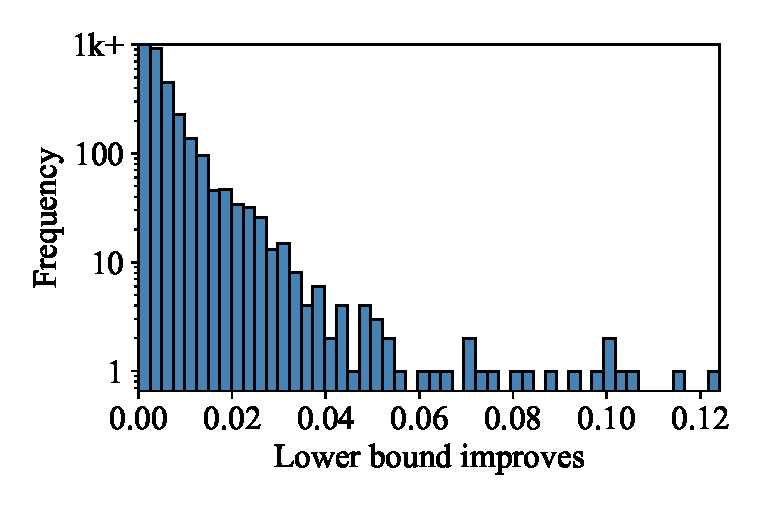
\includegraphics[width=\textwidth]{image/improves_1_255.eps}
      \caption{Improvements with $\varepsilon=\frac{1}{255}$}
      \label{fig:yolo_1_255}
    \end{subfigure}
    \hfill % 用于两幅图像之间的空间
    \begin{subfigure}[t]{0.32\textwidth}
      \centering
      \includegraphics[width=\textwidth]{image/improves_2_255.eps}
      \caption{Improvements with $\varepsilon=\frac{2}{255}$}
      \label{fig:yolo_2_255}
    \end{subfigure}
    \hfill % 用于两幅图像之间的空间
    \begin{subfigure}[t]{0.32\textwidth}
      \centering
      \includegraphics[width=\textwidth]{image/small_network.eps}
      \caption{Improvements in CNNs~\citep{cohen2024verification}}
      \label{fig:small_network}
    \end{subfigure}
    \caption{Verification bound improvement after Part 3}
    \label{fig:total refine}
\end{figure}


\begin{figure}[!t]
    \centering
    \begin{subfigure}[t]{0.48\textwidth}
      \centering
      \includegraphics[width=\textwidth]{image/image378.png}
      \caption{Image 378}
      \label{fig:img378}
    \end{subfigure}
    \hfill % 用于两幅图像之间的空间
    \begin{subfigure}[t]{0.48\textwidth}
      \centering
      \includegraphics[width=\textwidth]{image/image397.png}
      \caption{Image 397}
      \label{fig:img397}
    \end{subfigure}
    \caption{The effect of Part 3 in small object detection. The middle panel shows the bound from prior methods; the right panel shows our improved bound.}
    \label{fig:small refine}
  \end{figure}
This section shows that Part 3 in Section \ref{idea} and Appendix~\ref{app:part3} is effective for both large-scale networks (YOLO) and small-scale CNNs. %\ref{app:part3}
For the LARD dataset, we use a six-layer CNN network provided in \citep{cohen2024verification}.
As seen in Figure~\ref{fig:small_network}, with Part 3, the IoU lower bound we obtain is higher than the bound obtained without using Part 3. This improvement occurs because Part 3 reduces the over-approximation of the network's output, implying our bound is closer to the true bound. Note that we use sound formal verification on small object detection, instead of probabilistic verification, so that the network can indeed achieve such a bound.
For YOLO, we also show the effect of Part 3 in Fig. \ref{fig:yolo_1_255} and Fig. \ref{fig:yolo_2_255}. After refinement, most of the lower bounds are improved, which means Part 3 is also helpful in YOLO networks.

We observe that the first iteration yields the most significant gains. Since further refinement linearly accumulates confidence loss as described in Theorem 2, employing $T=1$ represents a favorable trade-off in most cases.

\section{Time Comparison}
\label{app:time comparison}
\begin{figure}[t]
\centering
\includegraphics[width=0.9\textwidth]{image/verification_time_comparison.pdf}
\caption{Verification time comparison}
\label{fig:verification_time_comparison}
\end{figure}

Fig.~\ref{fig:verification_time_comparison} shows the detailed time comparison of our method and $\mathrm{RCP}_N$ on different YOLO models with $\varepsilon=\frac{1}{255}$ and $\varepsilon=\frac{2}{255}$. The results show that our method is significantly faster than $\mathrm{RCP}_N$ in all images. 

\section{Real-world examples.} 
\label{app:real world}
\begin{table}[t]
\centering
\caption{Real world examples of our method.}
\label{tab:real world}
\begin{tabular}
{cccccccc}
\toprule
\multirow{2}{*}{model} & \multirow{2}{*}{$\varepsilon$} & \multirow{2}{*}{method} & \multirow{2}{*}{time} & \multicolumn{2}{c}{$\Delta_{\mathrm{PGD}}$} & \multicolumn{2}{c}{CRA}\\
 &  &  &  & ${\tau=0.5}$ & ${\tau=0.7}$ & ${\tau=0.5}$ & ${\tau=0.7}$\\
\midrule
\multirow{4}{*}{yolo11x}  & \multirow{2}{*}{1/(3 * 255)}  & $\mathrm{RCP}_{N}$  & 571.0  & 0.53  & 0.52  & \textbf{1.00}  & \textbf{1.00} \\ 

 &  & ODPV  & \textbf{32.1}  & \textbf{0.47}  & \textbf{0.44}  & \textbf{1.00}  & \textbf{1.00} \\ 
\addlinespace
 & \multirow{2}{*}{2/(3 * 255)}  & $\mathrm{RCP}_{N}$  & 569.6  & 0.57  & 0.55  & \textbf{1.00}  & \textbf{1.00} \\ 

 &  & ODPV  & \textbf{32.1}  & \textbf{0.43}  & \textbf{0.37}  & \textbf{1.00}  & \textbf{1.00} \\ 
\bottomrule
\end{tabular}
 
\end{table}

We take 40 images from sensor cameras of our autonomous vehicles and annotated ground truth by ourselves.
Table~\ref{tab:real world} shows the results of our method on these images. The results show that our method can also work well in real-world scenarios. Our method still uses less time and achieve better bounds than $\mathrm{RCP}_N$. Both CRA are high in these images, which means most boxes verified as robust by our method are reasonably robust.



\section{Compared with Median Smoothing}
\label{app:median}

\begin{table}[t]
\centering
\caption{Comparison of our method with median smoothing. $\Delta_{\mathrm{PGD}}$ denotes the mean absolute difference of IoU lower bounds relative to the PGD attack. Bold values indicate the best performance.}
\label{tab:median}
\begin{tabular}
{lcccccc}
\toprule
\multirow{2}{*}{model} & \multirow{2}{*}{$\varepsilon$} & \multirow{2}{*}{method} & \multicolumn{2}{c}{$\Delta_{\mathrm{PGD}}$} & \multicolumn{2}{c}{CRA}\\
 &  &  & ${\tau=0.5}$ & ${\tau=0.7}$ & ${\tau=0.5}$ & ${\tau=0.7}$\\
\midrule
\multirow{6}{*}{yolo11x}  & \multirow{3}{*}{1/255}  & $\mathrm{RCP}_{N}$  & 0.45  & 0.47  & \textbf{1.00}  & \textbf{1.00} \\ 

 &  & ODPV  & \textbf{0.42}  & \textbf{0.40}  & 0.99  & 0.98 \\ 

 &  & MS  & 0.44  & 0.45  & 0.99  & 0.98 \\ 
\addlinespace
 & \multirow{3}{*}{2/255}  & $\mathrm{RCP}_{N}$  & 0.59  & 0.56  & \textbf{1.00}  & \textbf{1.00} \\ 

 &  & ODPV  & \textbf{0.54}  & \textbf{0.47}  & \textbf{1.00}  & \textbf{1.00} \\ 

 &  & MS  & 0.59  & 0.53  & 0.96  & 0.97 \\ 
\bottomrule
\end{tabular}

\end{table}

Table~\ref{tab:median} compares our method with median smoothing (MS)~\citep{cohen2019certified} under normal distribution on 50 images from the COCO dataset. We set the standard deviation of normal distribution as $\sigma=\frac{1}{255 \times 3}$ and $\sigma=\frac{2}{255 \times 3}$. The results show that our method significantly achieves a smaller mean absolute difference of IoU lower bounds relative to the worst-case input found by the PGD attack($\Delta_{\mathrm{PGD}}$), indicating more precise IoU lower bounds. Besides, in most cases, the CRA of our method is higher than median smoothing. This also prove that our method works well in different distributions.

\section{Ablation Study of Parameters}
\label{app:ablation}
\begin{figure}[t]
\centering
\includegraphics[width=0.9\textwidth]{image/ablation_heatmaps.pdf}
\caption{Ablation study of parameters $\eta$, $\iota$}
\label{fig:ablation}
\end{figure}

Fig.~\ref{fig:ablation} shows the ablation study of parameters $\eta$ and $\iota$. The results show that our method still maintains more accurate bounds than $\mathrm{RCP}_N$ under different parameters. Besides, the results show that a larger $\eta$ and a larger $\iota$ will lead the bounds to be closer to the worst-case bound found by PGD attack. This is because a larger $\eta$ and a larger $\iota$ will results in a stricter NMS condition, fewer boxes can remain and the resulting boxes will be more robust.


\section{Broader Impact}
\label{app:border}

Our method focuses on verifying the safety of the object detection model, which may help people to better understand the model and give a safety metric. We do not think there is a negative social impact of our method as our method is not used to attack the model. 


\section{LLM Usage Statement}
\label{app:llm}
In the preparation of this manuscript, a Large Language Model (LLM) was utilized as a writing assistance tool. Its use was strictly confined to language polishing, which includes proofreading for grammatical errors, improving sentence structure, and enhancing the overall clarity and readability of the text.

All core intellectual contributions—including the research ideation, paper structure, and the initial drafting of the content—are the original work of the authors. The LLM did not contribute to the formulation of any hypotheses, experimental results, or conclusions presented herein. The authors have reviewed all AI-generated suggestions and take full responsibility for the final content of this paper.

\section{Description of hyperprameters}
\label{app:hyperprameters}

Our framework consists of three parts (Algorithms 1-4): Part 1 (Output Approximation), Part 2 (NMS Verification), and Part 3 (Counterexample-Based Refinement). Only Parts 1 and 3 are probabilistic; Part 2 is based on sound MIQP constraints and introduces no additional probabilistic error.

\subsection{Role of Parameters and Failure Events}
\begin{itemize}
    \item \textbf{$\alpha$ (Error Rate)}
    \begin{itemize}
        \item Appears in Definition~\ref{def: od_verification_problem_1} (OD PAC-Verification), Proposition~\ref{prop: prob_guaranee_for_part_1_1} (Part 1), Theorem~\ref{theorem: part_3_guarantee_1} (Part 3), and Theorem~\ref{theorem: full_guarateen_2} (Overall Guarantee).
        \item Controls the \emph{allowable violation probability} of the OD property under the input distribution: In Theorem~\ref{theorem: full_guarateen_2}, if the algorithm returns ``safe'' after at most $T$ refinement steps, we guarantee
        \[
        \mathrm{P}_{\boldsymbol{x}\sim \mathcal{C}}(\boldsymbol{x}\text{ is safe}) > 1 - (1+T)\,\alpha.
        \]
        \item In our experiments, we set $\alpha = 0.0099$, so with $T = 1$ we obtain a lower bound on the safety probability for each certified box of approximately $1 - 0.0198 \approx 0.98$.
    \end{itemize}

    \item \textbf{$\beta$ (Significance / Confidence)}
    \begin{itemize}
        \item Used for the scenario-type bounds in Part 1 (Prop.~\ref{prop: prob_guaranee_for_part_1_1}) and Part 3 (Thm.~\ref{theorem: part_3_guarantee_1}), and combined in Theorem~\ref{theorem: full_guarateen_2}.
        \item Controls the \emph{confidence} with which the above probabilistic claim holds, i.e., the probability that the inequality regarding $\mathrm{P}(\boldsymbol{x}\text{ is safe})$ is valid under the randomness of our sampling process. Theorem~\ref{theorem: full_guarateen_2} gives the overall confidence:
        \[
        \mathrm{P}\left[\mathrm{P}_{x\sim \mathcal{C}}(\boldsymbol{x}\text{ is safe}) > 1-(1+T)\alpha\right]
        \ge 1 - T\big(e^{-2N\delta^2} + \beta + 2(1-\epsilon)M_2\big) - \beta.
        \]
        \item We use $\beta = 0.0099$; with our default $N$, $\delta, \epsilon, M_2$, and $T = 1$, this lower bound is $\approx 0.98$ (reported in Appendix~\ref{app:exp details}).
    \end{itemize}

    \item \textbf{$\delta$ (Concentration slack in Part 3)}
    \begin{itemize}
        \item Appears only in Theorem~\ref{theorem: part_3_guarantee_1} / Theorem~\ref{theorem: full_guarateen_2}. It is the slack term in the Hoeffding bound, controlling how many of the $N$ sampled points in Part 3 have ``good'' local neighborhoods (i.e., have sufficient neighbors within the interval $[B_{\mathrm{F}(\boldsymbol{x})}, A_{\mathrm{F}(\boldsymbol{x})}]$).
        \item The condition
        \[
        N((1-2\epsilon)M - \delta) \;>\; \frac{2}{\alpha}\ln\frac{1}{\beta} + 2 + \frac{2}{\alpha}\ln\frac{2}{\alpha}
        \]
        ensures that with probability at least $1-\beta$, enough sample points are ``good'' to apply the $\mathrm{RCP}_N$-style scenario bound to the refinement constant $C$.
        \item We fix $\delta = 0.1$ in all experiments (Appendix~\ref{app:exp details}).
    \end{itemize}

    \item \textbf{$\epsilon$ (width of the local uncertainty interval in Part 3)}
    \begin{itemize}
        \item Used in Theorem~\ref{theorem: part_3_guarantee_1} to define the probability mass of the local distance interval $[B_{\mathrm{F}(\boldsymbol{x})}, A_{\mathrm{F}(\boldsymbol{x})}]$. For each $\boldsymbol{x}$, at least a $1-2\epsilon$ fraction of the $M$ local perturbations fall into this interval.
        \item The term $2(1-\epsilon)M_2$ in Theorem~\ref{theorem: full_guarateen_2} bounds the probability that the empirical estimation of this interval fails.
        \item We set $\epsilon = 1/200$ in all experiments.
    \end{itemize}
\end{itemize}

In practice, one needs to select appropriate $\alpha, \beta, \delta, \epsilon$ based on the desired probability thresholds and then calculate the sample sizes $N_1, N_2, N, M, M_2$. Below we discuss the relationship between sample sizes and these parameters.

\subsection{Sample Size Relationships}
The main sample size constraints appear in Theorem~\ref{theorem: full_guarateen_2}:

\begin{itemize}
    \item \textbf{Part 1 Sampling:}
    \[
    N_2 \ge \frac{2}{\alpha}\ln\frac{1}{\beta} + 2 + \frac{2}{\alpha}\ln\frac{2}{\alpha}.
    \]
    For fixed $\alpha, \beta$, we have $N_2 = O\!\big(\frac{1}{\alpha}\log\frac{1}{\beta}\big)$. Importantly, there is \textbf{no explicit dependency on the output dimension $d_L$} in this bound.

    \item \textbf{Part 3 Sampling:}
    With fixed $\delta, \epsilon, M$, the bound on $N$ can be written as
    \[
    N \;\ge\; \frac{1}{(1-2\epsilon)M-\delta}
    \Big( \frac{2}{\alpha}\ln\frac{1}{\beta} + 2 + \frac{2}{\alpha}\ln\frac{2}{\alpha} \Big),
    \]
    Thus, for fixed $\delta, \epsilon, M$, we again have $N = O\!\big(\frac{1}{\alpha}\log\frac{1}{\beta}\big)$.
\end{itemize}

In the experiments, we instantiate these quantities with the following values:
\[
N_1 = 30{,}000, \quad N_2 = 5{,}000, \quad N = 3{,}000, \quad M = 10, \quad M_2 = 2{,}000,
\]
and $\alpha = \beta = 0.0099$, $\epsilon = 1/200$, $\delta = 0.1$ (Appendix N). Because the samples from Part~1 are reused in Part~3 (Remark~\ref{remark: 5}), the total number of samples per box is:
\[
N_{\text{total}} = N_1 + N_2 + M_2 = 37{,}000
\]
This quantity is independent of $d_L$ and forms the basis for the claim ``achieving 98\% guarantee at 98\% confidence with 37,000 samples'' in Section~\ref{section: experiment}.

\subsection{Notation for sampling parameters}

Throughout Proposition~\ref{prop: prob_guaranee_for_part_1_1},
Theorem~\ref{theorem: part_3_guarantee_1} and
~\ref{theorem:  full_guarateen_2}, the symbols
$N_1,N_2,N,M,M_2,A'_i,B'_i,A_m,B_m$ and $C$ are inherited from
Algorithms~\ref{algforp1} and~\ref{algforp3} as follows.
In Algorithm~\ref{algforp1}, $N_1$ denotes the number of samples
used to estimate the per-coordinate scale vector $\boldsymbol{v}_{\max}$,
and $N_2$ is the number of samples used to compute the smallest
scaling factor $c_1$ in the optimization problem~\eqref{RC1}, which
yields the output hyper-rectangle $\mathcal{Z}$.
In Algorithm~\ref{algforp3}, $N$ is the number of reference points
$\{\boldsymbol{x}^{(i)}\}_{i=1}^N$ drawn from $\mathcal{C}$ in Step~One,
and $M$ is the number of auxiliary samples
$\{\boldsymbol{x}^{(i,j)}\}_{j=1}^M$ drawn for each reference point.
For each $i\in[N]$, we define
$A'_i=\max_{j\in[M]}\|\F(\boldsymbol{x}^{(i,j)})-\F(\boldsymbol{x}^{(i)})\|_2$
and
$B'_i=\min_{j\in[M]}\|\F(\boldsymbol{x}^{(i,j)})-\F(\boldsymbol{x}^{(i)})\|_2$,
and the constant $C$ is updated as
$C\gets \max\{C, B'_i/(A'_i-B'_i)\}$.
In Step~Two of Algorithm~\ref{algforp3}, $M_2$ denotes the number of
additional samples $\{\boldsymbol{x}^{(i)}\}_{i=1}^{M_2}$ drawn from
$\mathcal{C}$ to estimate the distance from a candidate output
$\boldsymbol{y}$ to the true output set $\{\F(\boldsymbol{x})\}_{\boldsymbol{x}\in\mathcal{C}}$,
with
$A_m=\max_{i\in[M_2]}\|\F(\boldsymbol{x}^{(i)})-\boldsymbol{y}\|_2$ and
$B_m=\min_{i\in[M_2]}\|\F(\boldsymbol{x}^{(i)})-\boldsymbol{y}\|_2$.
These quantities are then combined to form the estimator
$d_{\min}=\max\{(B_m-C(A_m-B_m))/(1+2C),0\}$ used in Part~3.

\section{Extending Our Method}
\label{app: other_attack}

We acknowledge that different architectures and threat models may necessitate distinct verification strategies, making a universal solution challenging.
Nonetheless, for many common threats, our proposed method can be adapted by modifying only the encoding in Part 2, while keeping Parts 1 and 3 unchanged. The following describes how to adapt our method to verify two additional threats: class misidentification and false appearances.


\subsection{Extending to Class Misidentification}


\begin{algorithm}[htbp]
\caption{Soundness Class Misidentification Verification for NMS}
\label{alg:nms_verification_mis}
\begin{algorithmic}[1]
\Require
Constraints $\mathcal{Z} = \mathcal{H} \setminus \mathcal{S}$; input $\boldsymbol{x}$; output $\boldsymbol{y}$; ground truth $box_{\mathrm{gt}}$; confidence threshold $\iota$.
\Ensure
Calculate per-box upper bounds $\{\tau_{\mathrm{mis}}(i)\}_{i=1}^{n_{\boldsymbol{x}}}$ for class misidentification.
\State $\{\overline{\underline{box}}_i\}_{i=1}^{n_{\boldsymbol{x}}} \gets \Call{Construct\_Abstract\_Box}{\mathcal{Z}}$
\ForAll {$\overline{\underline{box}}_i \in \{\overline{\underline{box}}_k\}_{k=1}^{n_{\boldsymbol{x}}}$}
    \State $\tau_{\mathrm{mis}}(i) \gets 0$
    \Comment{Initialize upper bound for misidentification IoU of box $i$}
    \If {$\forall k \in [n] \setminus\{\mathrm{Class}(box_{\mathrm{gt}})\},\ \underline{p}_{i,\mathrm{Class}(box_{\mathrm{gt}})} \geq \overline{p}_{i, k}$}
        \State \textbf{continue}
        \Comment{Skip boxes that must match $box_{\mathrm{gt}}$ class (never misclassified w.r.t. this GT)}
    \EndIf
    \If {$\overline{c_{i}} \geq \iota$}
        \Comment{Box $i$ may pass the confidence threshold in some realization}
        \State $\tau_{\mathrm{mis}}(i) \gets \Call{IoU\_Upper\_Bounds}{\overline{\underline{box}}_i, box_\mathrm{gt}}$
        \Comment{Worst-case IoU to $box_{\mathrm{gt}}$ when $box_i$ is potentially of a wrong class}
    \EndIf
\EndFor
\State \textbf{return} $\{\tau_{\mathrm{mis}}(i)\}_{i=1}^{n_{\boldsymbol{x}}}$
\end{algorithmic}
\end{algorithm}


\textbf{Formalization of the property (bad Event):}
Given an input constraint set $\mathcal{C}$, if there exists an input $\boldsymbol{x} \in \mathcal{C}$ such that after processing by the network $\mathrm{F}$ and NMS module, the output set $\mathrm{N}(\mathrm{F}(\boldsymbol{x}))$ contains a predicted box $box_i$ that has an IoU $\ge \tau$ with some GT box $box_{\mathrm{gt}}$, but their predicted and GT classes do not match, we consider this a class misidentification. Formally:
$$
\exists \boldsymbol{x} \in \mathcal{C},\ \exists box_i \in \mathrm{N}(\mathrm{F}(\boldsymbol{x})),\ \exists box_{\mathrm{gt}}\in\mathcal{G}:\
\mathbb{I}(\mathrm{class}(box_i) \neq \mathrm{class}(box_{\mathrm{gt}})) \cdot \mathrm{IoU}(box_i, box_{\mathrm{gt}}) \ge \tau.
$$

We want to prove that class misidentification does \textbf{not} occur, which is the negation of the bad event, equivalently written as:
$$
\forall \boldsymbol{x} \in \mathcal{C},\ \forall box_i \in \mathrm{N}(\mathrm{F}(\boldsymbol{x})),\ \forall box_{\mathrm{gt}}\in\mathcal{G}:\
\mathbb{I}(\mathrm{class}(box_i) \neq \mathrm{class}(box_{\mathrm{gt}})) \cdot \mathrm{IoU}(box_i, box_{\mathrm{gt}}) < \tau.
$$

To this end, we can define a worst-case function:
$$
\Phi_{\mathrm{cls}}(\boldsymbol{x}) =
\max_{box_i \in \mathrm{N}(\mathrm{F}(\boldsymbol{x})),\, box_{\mathrm{gt}}\in\mathcal{G}}
\left( \mathbb{I}(\mathrm{class}(box_i) \neq \mathrm{class}(box_{\mathrm{gt}})) \cdot \mathrm{IoU}(box_i, box_{\mathrm{gt}}) \right),
$$
The property holds if and only if:
$\sup_{\boldsymbol{x} \in \mathcal{C}} \Phi_{\mathrm{cls}}(\boldsymbol{x}) < \tau.$

Let $\mathcal{Z}$ be the over-approximation of the pre-NMS network output range $\{\mathrm{F}(\boldsymbol{x})\}_{\boldsymbol{x}\in\mathcal{C}}$ obtained in Part 1.Since our NMS analysis in Part 2 is applied uniformly over all $y \in \mathcal{Z}$, we can compute an upper bound of $\mathbb{I}(\mathrm{class}(box_i) \neq \mathrm{class}(box_{\mathrm{gt}})) \cdot \mathrm{IoU}(box_i, box_{\mathrm{gt}})$ on $\mathcal{Z}$ over all possible predicted boxes and GT pairs:
$$
U_{\mathrm{cls}} =
\sup_{box_i \in \mathcal{Z}, box_{\mathrm{gt}}\in\mathcal{G}}
\left( \mathbb{I}(\mathrm{class}(box_i) \neq \mathrm{class}(box_{\mathrm{gt}})) \cdot \mathrm{IoU}(box_i, box_{\mathrm{gt}}) \right).
$$

If we can prove
$U_{\mathrm{cls}} < \tau,$
then it is impossible for any $\boldsymbol{x} \in \mathcal{C}$ and any prediction/GT pair to have an IoU $\ge \tau$ and a class mismatch. Thus, we can certify that no class misidentification occurs within $\mathcal{C}$, and the property is verified.

Algorithm~\ref{alg:nms_verification_mis} shows how to compute per-box upper bounds on the misidentification IoU in Part 2.

\subsection{Extending to False Appearances}


\begin{algorithm}[htbp]
\caption{Soundness False Appearance Verification for NMS}
\label{alg:nms_verification_fa}
\begin{algorithmic}[1]
\Require
Constraints $\mathcal{Z} = \mathcal{H} \setminus \mathcal{S}$; input $\boldsymbol{x}$; output $\boldsymbol{y}$; set of ground truth boxes $\mathcal{G}$; confidence threshold $\iota$.
\Ensure
Calculate per-box lower bounds $\{\tau_{\mathrm{FA}}(i)\}_{i=1}^{n_{\boldsymbol{x}}}$ on $\max_{box_{\mathrm{gt}} \in \mathcal{G}} \mathrm{IoU}(box_i, box_{\mathrm{gt}})$.
\State $\{\overline{\underline{box}}_i\}_{i=1}^{n_{\boldsymbol{x}}} \gets \Call{Construct\_Abstract\_Box}{\mathcal{Z}}$
\ForAll {$\overline{\underline{box}}_i \in \{\overline{\underline{box}}_k\}_{k=1}^{n_{\boldsymbol{x}}}$}
    \State $\tau_{\mathrm{FA}}(i) \gets 0$
    \Comment{Initialize lower bound for maximal IoU to GTs of box $i$}
    \If {$\overline{c_{i}} < \iota$}
        \State \textbf{continue}
        \Comment{Box $i$ can never become a high-confidence detection, ignore it for False Appearance}
    \EndIf
    \State $lb \gets 0$
    \Comment{Lower bound on $\max_{box_{\mathrm{gt}} \in \mathcal{G}} \mathrm{IoU}(box_i, box_{\mathrm{gt}})$}
    \ForAll {$box_{\mathrm{gt}} \in \mathcal{G}$}
        \State $lb_{\mathrm{gt}} \gets \Call{IoU\_Lower\_Bounds}{\overline{\underline{box}}_i, box_\mathrm{gt}}$
        \State $lb \gets \max(lb, lb_{\mathrm{gt}})$
        \Comment{Aggregate lower bounds to over-approximate $\max_{box_{\mathrm{gt}}} \mathrm{IoU}$}
    \EndFor
    \State $\tau_{\mathrm{FA}}(i) \gets lb$
\EndFor
\State \textbf{return} $\{\tau_{\mathrm{FA}}(i)\}_{i=1}^{n_{\boldsymbol{x}}}$
\end{algorithmic}
\end{algorithm}


\textbf{Formalization of the property (bad Event):}
Given an input constraint set $\mathcal{C}$, if there exists an input $\boldsymbol{x} \in \mathcal{C}$ and a predicted box $box_i \in \mathrm{N}(\mathrm{F}(\boldsymbol{x}))$ whose IoU with all GT boxes is less than $\tau$, we consider this a False Appearance:
$$
\exists \boldsymbol{x} \in \mathcal{C},\ \exists box_i \in \mathrm{N}(\mathrm{F}(\boldsymbol{x})),\
\forall box_{\mathrm{gt}}\in\mathcal{G},\ \mathrm{IoU}(box_i, box_{\mathrm{gt}}) < \tau.
$$

Equivalently, define the \textbf{maximum IoU} for each predicted box with all GT boxes:
$$
\mathrm{IoU}_{\max}(box_i, \boldsymbol{x}) = \max_{box_{\mathrm{gt}}} \mathrm{IoU}(box_i, box_{\mathrm{gt}}),
$$
The bad event can be written as:
$$
\exists \boldsymbol{x} \in \mathcal{C},\ \exists box_i \in \mathrm{N}(\mathrm{F}(\boldsymbol{x})):\
\mathrm{IoU}_{\max}(box_i, \boldsymbol{x}) < \tau.
$$

We want to prove "no false appearances occur," which is the negation of the bad event:
$$
\forall \boldsymbol{x} \in \mathcal{C},\ \forall box_i \in \mathrm{N}(\mathrm{F}(\boldsymbol{x})):\
\mathrm{IoU}_{\max}(box_i, \boldsymbol{x}) \ge \tau.
$$

We can further define:
$$
\Phi_{\mathrm{FA}}(\boldsymbol{x}) =
\min_{box_i \in \mathrm{N}(\mathrm{F}(\boldsymbol{x}))} \mathrm{IoU}_{\max}(box_i, \boldsymbol{x}),
$$
and the property holds if and only if
$\inf_{\boldsymbol{x} \in \mathcal{C}} \Phi_{\mathrm{FA}}(\boldsymbol{x}) \ge \tau.$

Algorithm~\ref{alg:nms_verification_fa} shows how to compute per-box lower bounds on the maximum IoU to GT boxes in Part 2.

For any given property, we first formalize the attack and verification objective as described in Section 3 and the process above. Then, as in Section 4 and above, we adapt Part 2 of the algorithm (e.g., by adjusting the MIQP constraints) based on the specific verification objective. We will add a discussion of these and other potential extensions in the revised manuscript, and specify how Part 2 of the algorithm should be modified for these two threats.



\subsection{Evaluation}


To assess the effectiveness of our proposed method under diverse noise conditions and threat types, we conduct experiments using four distinct noise models and verify the False Appearance (FA) detection performance of our YOLO11x model. We define a noise tensor $\mathbf{N}_x$ and set the perturbation magnitude to $\varepsilon = 1/255$. The specific noise distributions and their corresponding real-world motivations are outlined below:

\begin{itemize}
\item \textbf{Uniform}: $\mathbf{N}_x \sim \mathcal{U}(-\varepsilon, \varepsilon)$ (Quantization/Uncertainty).
\item \textbf{Gaussian}: $\mathbf{N}_x \sim \mathcal{N}(0, (\varepsilon/3)^2)$ (Sensor Readout Noise).
\item \textbf{Salt-and-Pepper}: $\pm\varepsilon$ impulse noise with $p=0.05$ (Transmission Faults).
\end{itemize}
We randomly select 10 images from the COCO validation set and apply each noise model with $\varepsilon = 1/255$ to generate noisy inputs. We then evaluate the FA detection verification performance of our YOLO11x model on these perturbed images. For each input, we draw $10^6$ samples from the corresponding noise distribution to approximate the ground truth. The results are summarized in the table below:

\begin{table}[htbp]
\centering
\caption{FA Detection Verification Performance under Diverse Noise Models}
\label{tab:fa_verification}
\begin{tabular}
{llccccc}
\toprule
Model   &Noise type      &$\mathrm{CAR}_{\text{FA}}$   &$\mathrm{TPR}_{\text{FA}}$   &$\mathrm{TNR}_{\text{FA}}$   &$\mathrm{FPR}_{\text{FA}}$   &$\mathrm{FNR}_{\text{FA}}$  \\
\midrule
yolo11x &gaussian         &100.00\%                     &92.31\%                      &100.00\%                     &0.00\%                       &7.69\% \\                      
yolo11x &salt and pepper &100.00\%                     &85.71\%                      &100.00\%                     &0.00\%                       &14.29\% \\                     
yolo11x &uniform         &100.00\%                     &92.31\%                      &100.00\%                     &0.00\%                       &7.69\%  \\                    
\bottomrule
\end{tabular}
\end{table}

A detection is considered positive if it remains robust under the corresponding noise model and negative otherwise. The results indicate that our method sustains a high Certified Accuracy Rate (CAR) across different noise types, demonstrating that it provides reliable guarantees under diverse real-world noise conditions and threat types. Moreover, the True Positive Rate (TPR) and True Negative Rate (TNR) remain consistently high, while the False Positive Rate (FPR) and False Negative Rate (FNR) stay low, underscoring the method's effectiveness in distinguishing between robust and non-robust detections.

Overall, these results demonstrate that our method remains reliable across heterogeneous noise distributions and diverse threat types. This confirms that the proposed framework is broadly applicable and provides trustworthy robustness guarantees under a wide range of real-world noise conditions. the algorithm (e.g., by adjusting the MIQP constraints) based on the specific verification objective. We will add a discussion of these and other potential